% !TeX encoding = UTF-8
% !TeX program = pdflatex
% !TeX spellcheck = eng_ENG

%Pubblico il seguente file per condividere con i miei compagni di corso la struttura da me 
%configurata per la tesi in medicina e chirurgia al Sant'Andrea  

\documentclass[a4paper, oneside]{sapthesis}

% Useful packages for functionality
\usepackage{microtype}
\usepackage[english]{babel}
\usepackage{imakeidx}
\usepackage[acronym]{glossaries}
\usepackage{graphicx}
\usepackage{caption} % Added missing caption package
\captionsetup{labelsep=quad} 
\usepackage{array}
\usepackage{ragged2e}
\usepackage[table]{xcolor}
\usepackage{hyperref}
\usepackage{blindtext}

% Bibliography setup using biblatex and biber
\usepackage[
backend=biber,
style=ieee, % You can change this style as per your preference
sorting=ynt
]{biblatex}
\addbibresource{bibliography.bib} % Ensure the .bib file exists and is correct

\usepackage{csquotes}
\usepackage{enumitem}
\usepackage{tikz}
\usepackage{comment}
\usepackage{tgtermes}
\usetikzlibrary{angles,quotes,intersections}
\usetikzlibrary{3d,perspective}
\usepackage{subcaption}
\tikzset{axis/.style={thick,-latex}}
\tikzset{vec/.style={thick,blue}}
\tikzset{univec/.style={thick,red,-latex}}
\usepackage{physics}
\usepackage{bm}
\usepackage{tikz-3dplot}
\usepackage{amsmath, slashed}
\usepackage{amsfonts}
\usepackage[linguistics]{forest} % Diagram package
\usepackage{algorithm}
\usepackage{algpseudocode}
\usepackage{float}

% Define custom colors
\definecolor{ocra}{rgb}{1, 0.8, 0}      % Ocra color (HEX: #ffcc00)
\definecolor{orange}{rgb}{0.922, 0.38, 0.24} % Orange color (HEX: #eb613d)
\definecolor{gray}{rgb}{0.75, 0.75, 0.75}    % Gray color (HEX: #C0C0C0)
\definecolor{red}{rgb}{0.545, 0, 0}     % Dark Red color (HEX: #8B0000)
\definecolor{blue}{rgb}{0, 0, 0.803}    % Blue color (HEX: #0000CD)
\definecolor{green}{rgb}{0, 0.502, 0}   % Green color (HEX: #008000)

\renewcommand{\arraystretch}{1.3} % Increase vertical spacing in the matrix

% Custom command fixes
\newcommand*{\belowrulesepcolor}[1]{% 
  \noalign{% 
  \kern-\belowrulesep \begingroup \color{#1}% 
  \hrule height\belowrulesep \endgroup \relax }%
}
\newcommand*{\aboverulesepcolor}[1]{% 
  \noalign{%
  \begingroup \color{#1}% 
  \hrule height\aboverulesep \endgroup \kern-\aboverulesep \relax }%
}

% Metadata for PDF
\hypersetup{pdftitle={TITOLO TESI}, pdfauthor={Nome Cognome}}
\title{TITOLO TESI}
\author{Nome Cognome}
\IDnumber{MATRICOLA}
\course{Laurea Magistrale in Medicina e Chirurgia}
\courseorganizer{Facoltà di Medicina e Psicologia}
\AcademicYear{2022/2023}
\advisor{Dott.\textsuperscript{ssa} Nome Cognome}
\customadvisorlabel{Relatrice}
\authoremail{email autore}
\copyyear{2024}
\thesistype{Tesi sperimentale retrospettiva monocentrica}
\examdate{24 Gennaio 2024}
% You can reduce the number of examiners if the title page looks cluttered
\examiner{Prof. Tizio} 
\examiner{Prof. Caio} 
\examiner{Prof. Sempronio}  
\examiner{Prof. ...}  
\examiner{Prof. ...} 

% Glossaries
\makeindex
\makeglossaries
\newglossaryentry{PROVA}
{
        name=NOME DELLA VOCE GLOSSARIO,
        description={DESCRIZIONE DELLA VOCE GLOSSARIO}
}

\newacronym{GLOSSARIO}{GLOSSARIO}{\gls{PROVA}}


% Content setup
\includeonly{Cap_1,Cap_2,Cap_3,Cap_4,Cap_5}
\newcommand{\Fig}[1]{[{\footnotesize \texttt{Fig.#1}}]}
\newcommand{\citfig}[1]{\ap{\scriptsize\textrm{(\textit{F#1})}}}

\begin{document}
\frontmatter
\maketitle
%\dedication{Dedicato a \\
%SCRIVI QUI LA DEDICA
%}

\begin{abstract}

\paragraph{Contesto}


\paragraph{Obbiettivi}


\paragraph{Metodi} 

\paragraph{Risultati}

\paragraph{Conclusione}

\end{abstract}
\tableofcontents
\listoffigures
\listoftables

\phantomsection
\addcontentsline{toc}{chapter}{Acronimi}
\printglossary[type=\acronymtype]

\mainmatter
\documentclass[main]{subfiles}
\begin{document}
\section{Introduction}
\label{intro}

\subsection{Previous Works}
In the context of S\&R\footnote{S\&R stands for Search and Rescue.} operations, 
the support of robots has become more and more extensive in recent years 
\cite{sr0, sr1} and in particular the necessity and advantages of using 
\textit{decentralized multi-agent} systems \cite{multiagent}. A particular field 
of S\&R missions focuses on high mountain scenarios, in which UAVs 
\footnote{UAV stands for Unmanned Aerial Vehicles.} are tasked with localizing 
avalanche victims. These missions involve the smart collaboration between UAVs 
and humans also developed in the context of European-founded projects such as 
the SHERPA one \cite{sherpa}.

\noindent\\Different types of sensors can be used to achieve the localization goal, but the 
fastest and most accurate ones are electromagnetic sensors, which can operate 
also in noisy environments \cite{sensors}. Among these, the ARTVAs\footnote{ARTVA 
stands for the Italian “Apparecchio di Ricerca dei Travolti in VAlanga”.} are the 
most commonly used in both human-conducted and robot-conducted operations.

\noindent\\
Many studies have analyzed and formulated strategies and algorithms in the 
particular context of S\&R operations using UAVs for avalanche victims 
\cite{main, precedente, pre-main}. Furthermore, in order to address 
the localization problem, the authors of \cite{similar-main} and 
\cite{first-model} propose a robocentric SLAM approach in the broader robotics 
context. Note that in \cite{similar-main} they also take into consideration the 
\textit{multiple victims} case.

\noindent\\Avalanche victims rescue missions are challenging with respect to 
other S\&R operations because of some challenging aspects. In particular, the 
time constraint is quite demanding since the survival chances of avalanche 
victims diminish rapidly with time. Victims buried under avalanches have a 93\% 
survival rate within the first 15 minutes, which drops to 25\% after 45 minutes 
due to hypothermia \cite{survival} and plateaus at 21\% from 60 min to 180 
minutes \cite{survival2}.

\noindent\\The common human-conducted avalanche victims S\&R technique using ARTVA 
technology relies on three phases. In the first phase, rescuers search for the 
first valid electromagnetic signal, which can be detected at distances ranging 
from 20 meters for single-antenna receivers to 80 meters for triple-antenna ones. 
In the second phase, rescuers are trained to interpret the magnetic field data 
and follow standard procedures in order to follow the magnetic field direction and 
find the victim's position. In the final phase, rescuers dig to save the buried 
individual.

\noindent\\Despite the effectiveness of this technique, it requires a significant amount of 
time due to the challenges of traversing avalanche terrain. Additionally, 
rescuers walking on unstable snow face the tangible risk of triggering a 
secondary avalanche \cite{first-model}. For these reasons, and given the 
additional advantage of typically not encountering obstacles in high mountain 
scenarios, the use of intelligent \textit{autonomous} UAVs results in a faster 
and safer search when compared to human rescuers, as shown in \cite{sr, sr2, sr3}.

\noindent\\Therefore, this work aims to build upon previous efforts to 
\textit{automate} and improve the efficiency of the second phase by developing a 
mathematical/algorithmic framework for solving the localization problem of not 
just one, but \textit{multiple avalanche victims}, using \textit{multiple 
decentralized} agents (UAVs). This approach aims to reduce computational 
complexity without sacrificing accuracy and convergence time.

\subsubsection{Magnetic Dipole Localization}
In the context of a single magnetic source, numerous studies have focused 
on the localization task; in \cite{single_closed_formula_position} 
a straightforward closed-form solution is found by leveraging the analytical 
expressions of the magnetic field vector and the magnetic gradient tensor, 
regardless of the singularity of the magnetic gradient tensor matrix.

\noindent\\In the field of TMI\footnote{TMI stands for Total Magnetic Intensity} 
gradient surveys, the acquisition of magnetic gradient tensor data 
has seen significant advancements.
In \cite{NSS_analysis2}, new methods have been 
developed for inverting gradient tensor surveys, 
for several elementary, but useful, models. 
These include point pole, line 
of poles, point dipole (sphere), line of dipoles (horizontal cylinder), thin and thick 
dipping sheets, sloping step, and contact models.
A key insight is the use of eigenvalues and associated eigenvectors of the magnetic
tensor to obtain the NSS \footnote{NSS stands for Normalized Source Strength.},
which is a particularly useful rotational invariant that peaks 
directly over 2D sources, and it is independent of magnetization 
direction.

\noindent\\The NSS has been employed not only in geological applications but also in the  
the detection, location, and classification of magnetic objects, such as naval 
mines, UXO, shipwrecks, archaeological artifacts, and buried drums \cite{NSS_analysis2}.

\noindent\\In \cite{NSS_formula_important}, the authors use the spatial relation between the 
magnetic target and observation points derived from the NSS for accurately locating 
a magnetic target, achieving nearly error-free results in the absence of noise.
In addition, methods that use the NSS for magnetic sources localization, for different models
and dimensions is done in \cite{NSS_single_different_dimensions}. 

\noindent\\
In \cite{NSS_single_localization}, a key aspect of the NSS is identified by the fact
that it is only dependent on the distance between the source and target position;
since an analytical expression of the magnetic gradient tensor and a closed-form 
localization formula are derived.

\noindent\\
In \cite{NSS_analysis} as well, it is stressed that the NSS is proportional 
to a constant normalized by the distance between observation and source. 
It is independent of magnetization direction and satisfies Euler’s homogeneity equation, 
this allows the authors to use Euler deconvolution of the NSS to estimate source location.  

\noindent\\
Instead, the more specific multi-magnetic source localization task 
has been a difficult problem and different strategies have been conducted.
\noindent
In recent years, many studies have performed an in-depth analysis of rotational 
invariants of the magnetic gradient tensor, such as \cite{multiple_plots} and 
\cite{multiple_real_plots_invariants}.
In the latter, a new method, named NED\footnote{NED stands for New Edge Detection} 
has been proposed, which is free from geomagnetic interference and provides 
abundant information, and it is compared with other methods such as the tilt angle 
(ratio of vertical to horizontal magnetic field components),
theta map, etc.

\noindent\\
In this context of detecting and localizing multiple dipole-like 
magnetic sources, the authors of \cite{multiple_DE_NSS_big_matrix} 
use the magnetic gradient tensor data:
the tilt angle is used to determine the number of sources, 
while the rotational-invariant NSS is used to estimate the horizontal coordinates. 
Then, they employ the DE algorithm to estimate the locations and moments of the sources.

\noindent\\
Lastly, the authors of \cite{multiple_spacecraft} use 
the principal invariants of the magnetic field gradient tensor
to determine the number and horizontal location of the magnetic sources, 
while Euler equations are used to compute the sources's depth.

\noindent\\
In our work, between all the different indicators in the literature,
we chose to employ the NSS in order to estimate the 
horizontal coordinates of the avalanche victims, 
since it is rotationally invariant and completely isotropic 
around the magnetic dipole.
We are not interested in estimating the burial depth of the victims,
even if \cite{not_import_formula_z} use a closed loop formula to find z,
it cannot be applied to the multiple sources case.


\subsubsection{Particle Swarm Optimization}
In this context of simultaneous localization of multiple magnetic 
dipole sources, like in this real-world application \cite{real_application}; 
different algorithms have been employed.
For instance, in \cite{DetectionMultiplMagnetiDipoleSources}, the authors
use a non-linear optimization method based on the Levenberg–Marquardt algorithm
to solve the problem, without prior knowledge of the number of 
dipoles in the 3-D detection region.

\noindent\\In this work, we propose the use of the PSO\footnote{PSO stands for Particle Swarm Optimization.} 
algorithm as a means to solve the multiple-sources localization task, 
which can be considered a continuous multi-modal optimization problem.

\noindent\\
The PSO\footnote{PSO stands for Particle Swarm Optimization.} algorithm 
was first introduced in 1995 \cite{PSO_original}, and it has since proven to be 
a simple but powerful tool for solving various optimization problems\cite{PSO_IMPORTANT},
among a lot of EAs \footnote{EA stands for Evolutionary Algorithm.}.
It has been used to solve various practical applications like simultaneous
localization of multiple odor sources \cite{12}, as well as detection of acoustic 
\cite{PSO_acustic}, thermal, or chemical/biological signals \cite{3}.
In the robotics field, it has not only been employed in source-seeking 
applications but also path-planning scenarios \cite{PSO_for_path_planning} and
deployment of communication networks \cite{PSO_for_communication}.

\noindent\\
In the standard PSO algorithm \cite{PSO_original}, a population of particles is 
randomly initialized to represent potential candidate solutions for the optimization problem. 
Each particle relies on two important pieces of information: its individual 
best solution, referred to as \textit{pbest}, and the global best across the entire population, 
referred to as \textit{gbest}. These two values guide the search direction of all particles 
over the search space. 
The evaluation of the \textit{pbest} for each particle and the \textit{gbest} for 
the entire population is determined by the function that needs to be optimized.

\noindent\\
However, when addressing continuous optimization problems with numerous local optima, 
classical optimization algorithms often require strict conditions 
and extensive computation times \cite{PSO_another}.
For this reason, the authors of  \cite{PSO_IMPORTANT} introduced a modified PSO algorithm 
where the original population is divided into multiple subpopulations, 
according to the order of particles.
The best particle within each subpopulation is recorded and then 
used in the velocity updating formula to replace 
the original global best particle of the entire population.
This strategy, based on the idea of multiple subpopulations, 
enables the algorithm to find several optima, including both
the global and local solutions, thanks to these distinct best particles
in each group.

\noindent\\
Both in the standard PSO \cite{PSO_original} and the multi-swarm modification \cite{PSO_IMPORTANT}
common limitations are the premature convergence of the algorithm 
and its tendency to become trapped in some local optima.
Instead in \cite{PSO_another}, the authors overcome these issue,
including the one of poor population diversity. 
They introduce a modification to \cite{PSO_IMPORTANT}, it is called 
ADPSO\footnote{ADPSO stands for Adaptive Dynamic Multi-Swarm Particle Swarm Optimization.}, 
and includes features for stagnation detection and spatial exclusion to mitigate these challenges. 
The dynamic division of the population into sub-swarms, 
coupled with a regrouping mechanism, avoids stagnation during the optimization process. 
Stagnant sub-swarms are rejuvenated with a newly generated particle, 
called the vitality particle, constructed from the historical information of the entire population. 
This approach maintains diversity and prevents sub-swarms from converging prematurely.

\noindent\\
The authors of \cite{PSO_another2} focus their attention to the 
exploration and exploitation aspects of the PSO algorithm, instead.
They enhance exploration and exploitation in a modified system,
named HCLPSO \footnote{HCLPSO stands for Heterogeneous Comprehensive 
Learning Particle Swarm Optimization.}, which divides the population 
into only two sub-swarms, one dedicated to exploitation and 
one dedicated to exploration. 
In the exploration-subpopulation, the solutions are generated by using the personal 
best experiences of the particles in the exploration subpopulation itself. 
In the exploitation subpopulation, the personal best experiences of the
entire swarm population are used to generate the solutions. 
In this way, since the exploration-subpopulation does not
learn from any particles in the other subpopulation, 
diversity is maintained in the exploration-subpopulation even when the 
exploitation-subpopulation converges prematurely.

\subsection{The ARTVA}
The ARTVA technology is composed of two different and easy switchable modalities: 
in \textit{receiver} mode, the instrument senses and processes the 
electromagnetic field emitted by the ARTVA \textit{transmitter} (carried by the 
avalanche victim).

\noindent\\
The magnetic field generated by the solenoid antenna of the instrument oscillates 
with a frequency of 457 kHz and its characteristics are defined in the standard 
ETS 300 718-1 \cite{eu_standard}, to ensure compatibility between different 
brands and models. To save batteries and facilitate detection, the magnetic field 
is transmitted in pulses of a tenth of a second every second \cite{first-model}.

\noindent\\
As will be discussed more in-depth in the following chapter, the magnetic field 
can be modeled as a three-dimensional vector field, which means that it assigns a 
certain intensity and direction to each point in space. Therefore, the main 
difference between different kinds of ARTVAs lies in \textit{"how much"} of this 
field they can measure. According to this criterion, the instruments can be 
divided into three different types \cite{first-model}:

\begin{itemize}
    \item ARTVAs \textit{with one reception antenna}: the oldest models, usually
 analog. The same antenna is used in both \textit{transmitter} and 
    \textit{receiver} mode. Therefore, only the projection of the magnetic field 
 on the antenna can be measured. This type of ARTVA is the most difficult to 
 use and the most time-consuming one.
    
    \item ARTVAs \textit{with two perpendicular reception antennas}: are based on 
 digital technology such as microprocessors. This type can measure only the 
 intensity and direction of the horizontal component of the field, only when 
 held in a horizontal position.
    
    \item ARTVAs \textit{with three mutually perpendicular reception antennas}: 
 also based on digital technology. Since these ARTVAs possess three 
 perpendicular antennas, they can measure the complete vector field. For this 
 reason, the instrument can be oriented w.r.t the magnetic field in any way.
\end{itemize}

\noindent\\
In this work, we will consider only new ARTVA transceivers (three antennas), 
which can achieve a search strip width in digital mode of 80 m and a maximum 
range in analog mode of 90 m \cite{manual}. Furthermore, it is important to point 
the transceiver in the direction of the avalanche, parallel to the slope. For 
this reason, in this work, two different types of trajectories have been 
considered.
\end{document}
\chapter{Electromagnetism}

The ARTVA instrument in transmitter and receiver 
mode is a magnetic dipole. In order to formulate 
a coherent mathematical model, it is necessary to 
report some results of electromagnetic theory. 
Firstly, we identify and name the fundamental 
electromagnetic physical quantities.

\begin{table}[h!]
    \centering
    \begin{tabular}{lll}
        \hline
        Symbol & Description & Units \\
        \hline
        $\mathbf{E}$ & Electric field intensity & V/m \\
        $\mathbf{D}$ & Electric displacement field & C/m$^2$ \\
        $\mathbf{H}$ & Magnetic field intensity & A/m \\
        $\mathbf{B}$ & Magnetic flux density & T \\
        $\mathbf{J}$ & Current density & A/m$^2$ \\
        $\mathbf{A}$ & Magnetic vector potential & V $\cdot$ s/m \\
        $\mathbf{m}$ & Magnetic vector moment & A $\cdot$ m$^2$ \\
        $\rho$ & Volume charge density & C/m$^3$ \\
        $\epsilon$ & Permittivity of the medium & F/m \\
        $\mu$ & Permeability of the medium & H/m \\
        $c$ & Speed of light in vacuum & m/s \\
        \hline
    \end{tabular}
    \caption{List of electromagnetic physical 
    quantities and their descriptions.}
    \label{tab:symbols}
\end{table}

\section{Maxwell's Equations}

We postulate Maxwell's equations in a simple 
(linear, isotropic, and homogeneous) medium in 
phasor notation \ref{Phasor Notation}, which have 
been discovered experimentally \cite{book-magnetism}:

\begin{align}
    \nabla \times \mathbf{E} &= -j\omega \mathbf{B} 
    \label{eq:curl_E} \\
    \nabla \times \mathbf{H} &= \mathbf{J} + j\omega 
    \epsilon \mathbf{E} \label{eq:curl_H} \\
    \nabla \cdot \mathbf{E} &= \frac{\rho}{\epsilon} 
    \label{eq:E} \\
    \nabla \cdot \mathbf{B} &= 0 \label{eq:B}
\end{align}

In these equations, the space-coordinate arguments 
have been omitted for simplicity. The fact that 
the same notations are used for the phasors as 
are used for their corresponding time-dependent 
quantities should create little confusion because 
we will deal exclusively with sinusoidal vector 
fields.

From Maxwell's equation \ref{eq:B}, we know that 
the magnetic flux density \(\mathbf{B}\) is solenoidal 
(zero divergence). Then, \(\mathbf{B}\) can be expressed 
as the curl of another vector field using the 
Null Theorem \ref{eq:null}, obtaining \ref{eq:B}:

\begin{equation}
    \mathbf{B} = \nabla \times \mathbf{A}
    \label{curlA}
\end{equation}

Also, \(\mathbf{B}\) relates to the magnetic field 
intensity \(\mathbf{H}\) through the permeability of 
the medium \(\mu\):

\begin{equation}
    \mathbf{B} = \mu \mathbf{H}
    \label{eq:BH}
\end{equation}

Another useful form of Maxwell's first equation 
\ref{eq:curl_E} can be found by substituting 
\ref{curlA}:

\begin{align}
    \nabla \times \mathbf{E} = - j \omega 
    (\nabla \times \mathbf{A}) &= -\nabla \times 
    j \omega \mathbf{A} \nonumber \\
    \nabla \times \left(\mathbf{E} + 
    j \omega \mathbf{A}\right) &= 0 \nonumber
\end{align}

Since the sum of vector fields is itself a vector 
field, \(\mathbf{E} + j \omega \mathbf{A}\) is a 
vector field, and we can define a \textbf{scalar} 
field, the electric potential \(V\), such that:

\begin{equation}
    \mathbf{E} + j \omega \mathbf{A} = -\nabla V
    \label{eq:V}
\end{equation}

If the curl of a vector field is zero, a scalar 
field exists whose gradient gives the vector field.

\subsection{Conservation of Charge Principle}

The principle of conservation of charge states 
that the net charge within a closed system remains 
constant over time, meaning no charge can be 
created nor destroyed \cite{book-magnetism}:

\begin{equation}
    \nabla \cdot \mathbf{J} = -\frac{\partial \rho}
    {\partial t}
\end{equation}

The current density \(\mathbf{J}\) is defined as:

\begin{equation}
    \mathbf{J} = N q \mathbf{u}
\end{equation}

where \(N\) is the number of charge carriers per 
unit volume, \(q\) is the charge of each carrier, 
and \(\mathbf{u}\) is the drift velocity of the 
charge carriers.

This means that if a current flows out of a volume, 
the charge density inside the volume must decrease 
at a rate equal to the current. The current leaving 
the volume is the flux of the current density 
through surface \(S\):

\begin{equation}
    I = \oint_S \mathbf{J} \cdot d\mathbf{s}
    \label{eq:defI}
\end{equation}

\section{Wave Equation for Magnetic Vector Potential}

In order to determine the intensity of the magnetic 
field, we first need to find an expression for the 
magnetic vector potential \(\mathbf{A}\), called the 
wave equation. Starting from Maxwell's equations, 
we find the wave equation by substituting \ref{curlA} 
and \ref{eq:BH} into the second Maxwell equation 
\ref{eq:curl_H}:

\[
    \nabla \times \nabla \times \mathbf{A} = 
    \mu \mathbf{J} + j\omega\epsilon \mu \mathbf{E}
\]

Then we substitute \ref{eq:V} for $\mathbf{E}$ and 
use the Laplacian \ref{eq:laplacian} on the left side:

\[
    \nabla (\nabla \cdot \mathbf{A}) - \nabla^2 
    \mathbf{A} = \mu \mathbf{J} + j\omega \epsilon 
    \mu \left(-\nabla V - j \omega \mathbf{A}\right)
\]

The definition of a vector requires the specification 
of both its curl and its divergence. Although the curl 
of $\mathbf{A}$ is designated $\mathbf{B}$ in 
\ref{curlA}, we are still at liberty to choose its 
divergence to simplify the expression 
\cite{book-magnetism}:

\[
    \nabla \cdot \mathbf{A} = - j \omega \epsilon 
    \mu V
\]

Finally, rearranging the terms and substituting 
the square of $j$, we get:

\[
    \nabla^2 \mathbf{A} + \omega^2 \epsilon \mu 
    \mathbf{A} = -\mu \mathbf{J}
\]

This is the wave equation for the magnetic vector 
potential \(\mathbf{A}\):

\begin{equation}
    \nabla^2 \mathbf{A} - k^2 \mathbf{A} = 
    -\mu \mathbf{J}
    \label{eq:wave}
\end{equation}

where \(k = \omega \sqrt{\mu \epsilon}\) is the wave 
number, which characterizes the propagation of the 
electromagnetic wave in the medium.
\subsection{Finding the Potential by Solving the Wave Equation}

Since both \(\mathbf{A}\) and \(\mathbf{J}\) are vector 
fields, the wave equation \ref{eq:wave} can be written 
for each component of \(\mathbf{A}\):

\begin{equation}
    \nabla^2 
    \begin{pmatrix} 
        A_x \\ A_y \\ A_z 
    \end{pmatrix} = 
    k^2 
    \begin{pmatrix} 
        A_x \\ A_y \\ A_z 
    \end{pmatrix} - 
    \mu 
    \begin{pmatrix} 
        J_x \\ J_y \\ J_z 
    \end{pmatrix}
    \label{eq:wavematrix}
\end{equation}

In order to solve \ref{eq:wavematrix}, we can use the 
Green function for Poisson's equation \ref{eq:poisson} 
for each of the components when $k = 0$ (the case of 
static fields). Then, the solution is given by the 
formula:

\begin{equation}
    \mathbf{A} = \frac{\mu}{4 \pi} \int_V 
    \mathbf{J} \frac{e^{-jkr}}{r} dv
    \label{eq:solA}
\end{equation}

by using the superposition principle and by finding the 
solution of the time-dependent differential equation.

\section{Magnetic Dipole}

\begin{figure}
    \centering
    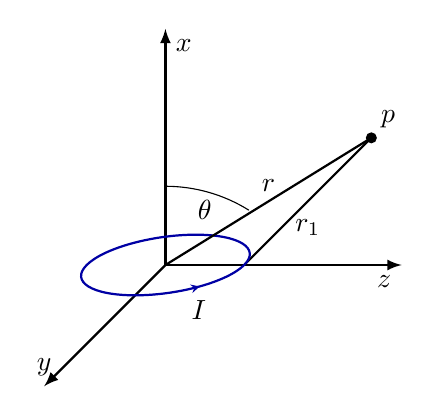
\begin{tikzpicture}
        % Draw the 3D coordinate system
        \draw[axis] (0,0,0) -- (3,0,0) 
        node[anchor=north east]{$z$};
        \draw[axis] (0,0,0) -- (0,3,0) 
        node[anchor=north west]{$x$};
        \draw[axis] (0,0,0) -- (0,0,4) 
        node[anchor=south]{$y$};
        % Coordinates
        \coordinate (O) at (0,0,0);
        \coordinate (R) at (3,2,1);
        % Line from p to b
        \draw[thick] (1,0,0) -- (R) 
        node[midway, below, yshift=-0.1cm]{$r_1$};
        % Draw the point r
        \fill (R) circle (2pt);
        \node[above right] at (R) {$p$};
        % Draw and label the angle theta
        \draw (0,1) arc[start angle=90,end angle=58,,radius=2cm];
        \node at (0.5,0.7) {$\theta$};
        % Label in space called b
        \node at (1,0,1.5) {$I$};
        % Draw a circle in the xz-plane
        \begin{scope}[canvas is xz plane at y=0]
            \draw[thick, color=blue!80!black] 
            (0,0) circle [radius=1];
            \draw[-stealth, color=blue!80!black] 
            (0,1) arc[start angle=90,end angle=45,radius=1];
        \end{scope}
        % Draw the line from origin to point r
        \draw[thick] (O) -- (R) node[midway, above]{$r$};
    \end{tikzpicture}
    \caption{Magnetic dipole representation}
    \label{fig:dipole}
\end{figure}

We have a small filament loop of radius \( b \), 
carrying an AC current \( I(t) = I \cos(\omega t) \) 
as shown in Figure \ref{fig:dipole}. If \( S \) is the 
cross-section area of the wire and \( dl \) a 
differential length, we have \( \mathbf{J} \perp 
\mathbf{s} \), the normal to the area and the volume:

\begin{equation}
    dv = S \, dl
    \label{eq:dvolume}
\end{equation}

In order to determine the magnetic field intensity 
\(\mathbf{H}\) at a certain point in space \( p \), 
we need to compute the magnetic vector potential 
\(\mathbf{A}\) first \cite{book-magnetism}. Since the 
charges move only in the thin wire, they are located 
only in the wire region, then from the definition of 
current \ref{eq:defI}:

\[
    I = S \, \mathbf{J}
\]

The volume integral in \ref{eq:solA} becomes:

\[
    \int_V \mathbf{J} \, dv =  \int_V \mathbf{J} \, S \, dl
\]

Then, we substitute \ref{eq:defI} and change the 
integral type since it is now the sum over the length, 
so the formula becomes (the current must flow in a 
closed path):

\begin{equation}
    \mathbf{A} = \frac{\mu_0 I}{4\pi} \oint_C 
    \frac{d\mathbf{l}}{r_1} e^{-j k r_1}
    \label{sol_A_dipole}
\end{equation}

where $r_1$ is the distance between the point $p$ and 
the charges (source element) and $d\mathbf{l}$ is a 
vector tangent to the loop of differential length $dl$.

\subsubsection{Assumption} \label{Assumption}

We can then simplify \ref{sol_A_dipole} by considering 
the radius $b$ to be small enough, such that 
$r_1 - r \approx 0$. Then by adding and subtracting $r$ 
from the power of the exponential:

\[
    e^{-j k r_1} = e^{-j k (r_1 + r - r)} = 
    e^{-j k r} \, e^{-j k (r_1 - r)}
\]

Then by using Taylor approximation on the second 
exponential ($ x = r_1 - r \approx 0$) we obtain:

\[
    e^{-j k r_1} = e^{-j k r}\, \left[ 1 - j k (r_1 - r) \right]
\]

Then, we substitute this result in \ref{sol_A_dipole} 
and simplify:

\[
\begin{aligned}
    \mathbf{A} &= \frac{\mu_0 I}{4 \pi} e^{-j k r} 
    \left[ 1 - j k (r_1 - r) \right] \oint_C 
    \frac{d\mathbf{l}}{r_1} \\
    &= \frac{\mu_0 I}{4 \pi} e^{-j k r} \left( 
    \oint \frac{d\mathbf{l}}{r_1} - j k \oint 
    (r_1 - r) \frac{d\mathbf{l}}{R_1} \right)
\end{aligned}
\]

Since the integral of \(d\mathbf{l}\) over a closed loop 
is zero, because we have considered a small loop $b \to 0$:

\[
    \oint_C d\ell = 2\pi b \quad \rightarrow \quad 
    \oint_C d\ell \rightarrow 0
\]

Then we obtain:

\begin{equation}
    \mathbf{A} = \frac{\mu_0 I}{4 \pi} e^{-j k r} 
    \left[ \left(1 + j k r \right) \oint 
    \frac{d\mathbf{l}}{r_1}\right]
    \label{eq:sol_A_simp}
\end{equation}
\subsubsection{Assumption Quasi-Static Field/Near Field Zone}
If we consider a region near the magnetic dipole, we 
obtain quasi-static fields. We defined the wave number 
$k$ as:

\begin{equation}
    k = \omega \sqrt{\mu \epsilon}
    \label{eq:k}
\end{equation}

Electromagnetic waves propagate with velocity $u$ 
(speed of light in vacuum) \cite{book-magnetism}:

\begin{equation}
    u = \frac{1}{\sqrt{\mu \epsilon}}
    \label{eq:u}
\end{equation}

Then, by inverting \ref{eq:u} and substituting in 
\ref{eq:k}, we can write $k$ as:

\begin{equation}
    k = \frac{\omega}{u}
    \label{eq:k2}
\end{equation}

From wave theory $f = \frac{\omega}{2\pi}$ and 
$\lambda = \frac{u}{f}$, we obtain another expression 
for $u$:

\begin{equation}
   u = \frac{\lambda \, \omega}{2 \, \pi}
\end{equation}
\label{eq:u2}

\noindent Therefore, we can substitute \ref{eq:u2} in 
\ref{eq:k2}:

\begin{equation}
    k = \frac{2 \pi}{\lambda}
    \label{eq:k3}
\end{equation}

To simplify the expression for $\mathbf{A}$ 
\ref{sol_A_dipole}, we make the assumption that 
$k \, r \ll 1$, and if we substitute the found 
expression of $k$ \ref{eq:k3}:

\[
    k \, r \ll 1 \implies \frac{2\pi r}{\lambda} 
    \ll 1 \implies r \ll \frac{\lambda}{2\pi}
\]

This means that $r$ needs to be small in comparison 
to $\lambda$. If this is the case:

\[
    e^{-j k r} \approx e^0 = 1
\]

We eliminate completely the time dependence and 
obtain the expression for $\mathbf{A}$:

\begin{equation}
    \mathbf{A} = \frac{\mu_0 I}{4\pi} \oint_C 
    \frac{d\mathbf{l}}{r_1}
    \label{A_approx}
\end{equation}

In the ARTVA case, the standard operating frequency 
is \( f = 475 \, \text{kHz} \) and the optimal range 
of the instrument is \( <80 \, \text{m} \). Then in 
the worst case, when \( r = 80 \, \text{m} \), we 
obtain the approximation \( k \, r = 0.79 \).

\subsubsection{Symmetry}

In the particular case of a magnetic dipole, the 
magnetic vector potential $\mathbf{A}$ is symmetric 
with respect to the \(x\)-axis, therefore independent 
to the $\phi$ angle \ref{Spherical Coordinates}. 
This is true since we can choose freely the $z$-axis 
and $y$-axis orientation in space around the loop. 
Then we can choose the point $\mathbf{p}$ to lie on 
the $zx$-plane or the $yx$-plane; in both cases, we 
will obtain that one of the two $d\mathbf{l}$ 
components $d\mathbf{l_z}$ and $d\mathbf{l_y}$ will 
cancel themselves out as we integrate over the loop.

For example, if we consider the point to lie on the 
$yx$-plane, then take a point on the loop where 
$d\mathbf{l}$ is and its symmetric w.r.t. the 
$y$-axis, the component $d\mathbf{l_y}$ of the first 
will cancel itself out with the one of the second.

We can write the length of a circumference as 
$l = r \, \alpha$, where $\alpha$ is the subtended 
angle by the length $l$ and $r$ the radius. In 
addition, we express $\mathbf{e_\phi}$ using the 
Cartesian basis:

$$
    \mathbf{e_\phi} = - \sin\phi \, \mathbf{e_y} 
    + \cos\phi \, \mathbf{e_z}
$$

Then, $d\mathbf{l}$ magnitude depends on the 
differential angle $d\phi$ and the radius $b$, and 
has the same direction as $\mathbf{e_\phi}$:

\begin{equation}
    d\mathbf{l} = b \, d\phi \, \mathbf{e_\phi} 
    = b \, d\phi \left(- \sin\phi \, \mathbf{e_y} 
    + \cos\phi \, \mathbf{e_z}\right)
    \label{eq:dl}
\end{equation}

For every $d\mathbf{l}$, there is another 
symmetrically located differential length element on 
the other side of the $y$-axis that will contribute 
an equal amount to $\mathbf{A}$ in the $\mathbf{e_z}$ 
direction but will cancel the contribution of 
$d\mathbf{l}$ in the $\mathbf{e_y}$ direction. 
Since $\mathbf{e_z} = \mathbf{e_\phi}$, if point $P$ 
lies on the $yx$-plane, equation \ref{A_approx} can 
be written as:

\begin{equation}
    \mathbf{A} = \mathbf{e_\phi} \frac{\mu I b}{4 \pi} 
    \int_{0}^{2\pi} \frac{\cos \phi}{r_1} \, d\phi
    \label{eq:A_final}
\end{equation}

\subsubsection{Computing the Integral in Spherical Coordinates}

Firstly, we find $r_1$ by applying the law of cosines 
on the triangle $OPP'$, Figure \ref{fig:dipole2}:

\begin{figure}
    \centering
    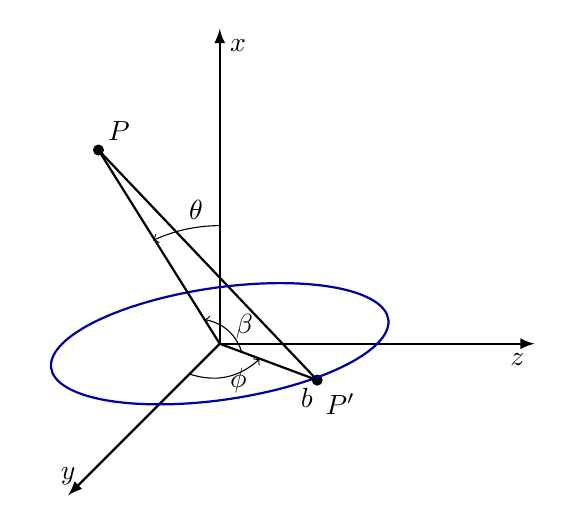
\begin{tikzpicture}
        % Draw the 3D coordinate system
        \draw[axis] (0,0,0) -- (4,0,0) 
        node[anchor=north east]{$z$};
        \draw[axis] (0,0,0) -- (0,4,0) 
        node[anchor=north west]{$x$};
        \draw[axis] (0,0,0) -- (0,0,5) 
        node[anchor=south]{$y$};
        % Coordinates
        \coordinate (O) at (0,0,0);
        \coordinate (R) at (0,4,4);
        \coordinate (P') at (1.7,0,1.2);
        % Line from p to b
        \draw[thick] (P') -- (R) node[right, yshift=0.1cm]{};
        % Draw the point 
        \fill (R) circle (2pt);
        \fill (P') circle (2pt);
        \node[above right] at (R) {$P$};
        % Draw the angle theta between r and y-axis
        \draw[->] (0,1.5,0) arc[start angle=90, 
        end angle=115, radius=2cm];
        \node at (-0.3,1.7,0) {$\theta$};
        \draw[bend right,->] (0,0,1) to 
        node [auto] {} (0.7,0,0.5);
        \node at (0.7,0.6,1) {$\beta$};
        \draw[bend right,->] (0.4,0,0.3) to 
        node [auto] {} (0,0.5,0.5);
        % Label in space called b
        \node at (1.8,0,1.8) {$b$};
        \node at (2.3,0,2) {$P'$};
        \node at (0.7,0,1.2) {$\phi$};
        % Draw a circle in the xz-plane
        \begin{scope}[canvas is xz plane at y=0]
            \draw[thick, color=blue!80!black] 
            (0,0) circle [radius=2];
        \end{scope}
        % Draw the line from origin to point r
        \draw[thick] (O) -- (R) 
        node[midway, above right, yshift=0.4cm]{};
        \draw[thick] (O) -- (P') 
        node[midway, above right]{};
    \end{tikzpicture}
    \caption{Magnetic dipole representation with the $OPP'$ triangle}
    \label{fig:dipole2}
\end{figure}

We start with the equation for \( r_1 \):
$$
    r_1^2 = r^2 + b^2 - 2 r b \cos\beta
$$
Since we are on the \( xy \)-plane, we can write the 
\( \mathbf{b} \) and \( \mathbf{r} \) vectors as:
$$
    \mathbf{r} = r \sin \theta \, \mathbf{e_y} 
    + r \cos \theta \, \mathbf{e_x}
$$
$$
    \mathbf{b} = b \cos \phi \, \mathbf{e_y} 
    + b \sin \phi \, \mathbf{e_z}
$$
Then we find the angle \(\beta\) between 
\( \mathbf{r} \) and \( \mathbf{b} \):
$$
    \cos \beta = \frac{\mathbf{b} \cdot \mathbf{r}}{r b} 
    = \sin \theta \cos \phi
$$
We have obtained a formula for \( r_1 \):
$$
    r_1 = \sqrt{r^2 + b^2 - 2 r b \sin \theta \cos \phi}
$$
Simplifying further, we get:
$$
    r_1^2 = r^2 \left( 1 + \frac{b^2}{r^2} - 2\, 
    \frac{b}{r} \sin \theta \cos \phi \right)
$$
Using the same assumption as before, that the loop is 
very small with respect to \( r \) (i.e., \( b \ll r \) 
and therefore \( b^2 \ll r^2 \)), we can write:
$$
    r_1 \approx r \left( 1 - 2 \, \frac{b}{r} \, 
    \sin \theta \cos \phi \right)^{1/2}
$$
Then we compute the inverse \( \frac{1}{r_1} \) and 
use the Taylor approximation to the first derivative, 
considering \( x = 2 \, \frac{b }{r} \, \sin \theta 
\cos \phi \), which tends to zero, we obtain:

\begin{equation}
    \frac{1}{r_1} \approx \frac{1}{r} 
    \left( 1 + \frac{b}{r} \sin \theta \cos \phi \right)
    \label{eq:r_1}
\end{equation}

Now, substituting \ref{eq:r_1} in \ref{eq:A_final}, we 
can calculate the integral for \( \mathbf{A} \) over 
the entire loop:

$$
    \mathbf{A} = \mathbf{e_\phi} \frac{\mu I b}{4 \pi} 
    \int_{0}^{2\pi} \left( 1 + \frac{b}{r} \sin \theta 
    \cos \phi \right) \cos \phi \, d\phi
$$

Since \( b \), \( r \), and $\theta$ do not depend on 
$\phi$, the first integral is zero, and the second one 
gives $\pi$:

\begin{enumerate}[label=(\arabic*)]
    \item 
    \parbox{\textwidth}{
    \[
        \int_0^{2\pi} \cos \phi \, d\phi = \sin \phi \Big|_0^{2\pi} = 0
    \]
    }

    \item 
    \parbox{\textwidth}{
    \[
        \int_{0}^{2\pi} \cos^2 \phi \, d\phi = \int_{0}^{2\pi} 
        \frac{1 + \cos(2\phi)}{2} \, d\phi = \frac{1}{2} \cdot 2\pi 
        + \frac{1}{2} \cdot 0 = \pi
    \]
    }
\end{enumerate}

Therefore, we obtain:

\begin{equation}
    \mathbf{A} = \mathbf{e_\phi} \frac{\mu I b^2}{4 \, r^2} 
    \sin \theta
    \label{eq:A_spher}
\end{equation}

\subsubsection{Magnetic Field Intensity $\mathbf{H}$}
Finally, we can now obtain an expression in spherical 
coordinates of the magnetic field intensity 
$\mathbf{H}$, by first finding $\mathbf{B}$ using 
\ref{curlA} and then inverting \ref{eq:BH}.
\\
We compute the curl of $\mathbf{A}$ in spherical 
coordinates \ref{curl_spher}:

\[
    \mathbf{B} = \nabla \times \mathbf{A} = \frac{1}{r^2 \sin \theta} 
    \begin{vmatrix}
        \mathbf{e_r} & \mathbf{e_\theta} r & \mathbf{e_\phi} r \sin \theta \\
        \frac{\partial}{\partial r} & \frac{\partial}{\partial \theta} & 
        \frac{\partial}{\partial \phi} \\
        0 & 0 & r \sin \theta A_\phi
    \end{vmatrix} =
\]
\[
    = \frac{1}{r^2 \sin \theta} \left( \mathbf{e_r} 
    \frac{\partial}{\partial \theta} (r \sin \theta A_\phi) 
    - \mathbf{e_\theta} \frac{\partial}{\partial r} 
    (r \sin \theta A_\phi) \right)
\]

where $A_\phi$ is the magnitude of the vector field 
found in \ref{eq:A_spher}, while $A_r$ and $A_\theta$ 
are zero since the potential has only the 
$\mathbf{e_\phi}$ direction. Substituting 
\ref{eq:A_spher}:

\[
\begin{aligned}
    \mathbf{B}&= \frac{1}{r^2 \sin \theta} 
    \frac{\mu b^2 I}{4 \pi} \left(\mathbf{e_r} 
    \frac{2}{r} \cos \theta \sin \theta + 
    \mathbf{e_\theta} r \sin^2 \theta \, r^{-2}\right) =
    \\
     &= \frac{\mu I b^2 }{4 \, r^3} \left( 
     \mathbf{e_r} 2 \cos \theta + \mathbf{e_\theta} 
     \sin \theta \right)
\end{aligned}
\]

Then, by inverting equation \ref{eq:BH}, we obtain the 
final expression for $\mathbf{H}$:

\begin{equation}
    \mathbf{H} = \frac{ I b^2}{4 \, r^3} \left( 
    \mathbf{e_r} 2 \cos \theta + \mathbf{e_\theta} 
    \sin \theta \right)
    \label{eq:H_spheric}
\end{equation}

which can also be expressed using the Cartesian unit 
vectors \((\mathbf{e}_x, \mathbf{e}_y, \mathbf{e}_z)\) 
by substituting \(\mathbf{e}_r\) with \ref{e_r} and 
\(\mathbf{e}_\theta\) with \ref{e_theta}:

\[
    \mathbf{H} = \frac{I b^2}{4 \pi \, r^3} \left[ 
    (2\cos^2\theta - \sin^2\theta) \mathbf{e}_x 
    + 3\cos\theta \sin\theta \cos\phi \, \mathbf{e}_y 
    + 3\cos\theta \sin\theta \sin\phi \, \mathbf{e}_z \right]
\]

or in vector form:

\[
    \mathbf{H} = \frac{I b^2}{4 \, r^3} 
    \begin{bmatrix}
        2\cos^2\theta - \sin^2\theta \\
        3\cos\theta \sin\theta \cos\phi \\
        3\cos\theta \sin\theta \sin\phi
    \end{bmatrix}
\]

We can finally find the expression for $\mathbf{H}$ 
using only Cartesian coordinates by inverting the 
equations in \ref{Conversion from Spherical to 
Cartesian Coordinates}:

\begin{equation}
    \mathbf{H} = \frac{I b^2}{4 \, r^5} 
    \begin{bmatrix}
        2x^2 - y^2 - z^2 \\
        3xy \\
        3xz
    \end{bmatrix}
\label{eq:final_H}
\end{equation}

This expression has been derived by applying the Pythagorean identity.

\section{Normalized Source Strength}
The magnetic field intensity $\mathbf{H}$ and the magnetic flux density $\mathbf{B}$ are vector fields 
sensible to the orientation of the source coordinate system. 
The expression for $\mathbf{H}$, as given in equation \ref{eq:final_H}, is expressed with respect to a 
coordinate system centered at the center of the current loop, as we have seen in the previous section.
However, we need to introduce a quantity which is invariant with
respect to the orientation of the electromagnetic target.
Many studies have conducted in-depth analysis on rotational invariants of the magnetic gradient tensor,
such as \cite{multiple_plots} and \cite{multiple_real_plots_invariants}.
The magnetic gradient tensor is simply the transposed Jacobian of the magnetic flux density $\mathbf{B}$, and it is defined
as follows:
\begin{equation}
\begin{aligned}
\mathbf{G} &= 
\begin{bmatrix}
    \frac{\partial B_x}{\partial x} & \frac{\partial B_y}{\partial x} & \frac{\partial B_z}{\partial x}\\
    \frac{\partial B_x}{\partial y} & \frac{\partial B_y}{\partial y} & \frac{\partial B_z}{\partial y}\\
    \frac{\partial B_x}{\partial z} & \frac{\partial B_y}{\partial z} & \frac{\partial B_z}{\partial z}\\
\end{bmatrix}
\\
&=
\begin{bmatrix}
    B_{xx} & B_{yx} & B_{zx}\\
    B_{xy} & B_{yy} & B_{zy}\\
    B_{xz} & B_{yz} & B_{zz}\\
\end{bmatrix}
\end{aligned}
\label{eq:Jacobian}
\end{equation}
It represents the spatial rate of change of the magnetic field vector $\mathbf{B}$
along the three mutually orthogonal directions of the Cartesian coordinates.

In most cases, rotational invariants,
such as the Frobenius norm of $\mathbf{G}$ and any combination of its
eigenvalues, are sensitive to the direction of the target magnetic
moment vector $\mathbf{m}$ \cite{NSS_single_localization}. The magnetic moment represents the strenght 
and orientation of the magnetic field, and for a magnetic dipole of a current
loop it is defined as follows, \cite{book-magnetism}:
\begin{equation}
    \mathbf{m} = I \, \mathbf{S}
\end{equation}
where $I$ is the current flowing in the loop and $\mathbf{S}$, is the normal to the area of the loop
and it is not to be confused with $S$ in \ref{eq:dvolume}, which is the area
of the section of the wire.
In our representation of the magentic dipole, with the Cartesian axes
defined in Figure \ref{fig:dipole}, the direction of the magnetic moment is the $x$-axis,
and the magnitude is:
\begin{equation}
    m = I \, \pi \, b^2
    \label{eq:magnetic_moment}  
\end{equation}

Instead the NSS\footnote{NSS stands for Normalized Source Strength}, a tensor invariant calculated 
from the eigenvalues of the magnetic gradient tensor $\mathbf{G}$, 
does not depend on the magnetization direction and it 
is completely isotropic around the magnetic dipole \cite{multiple_real_plots_invariants}.
This follows from the magnetic gradient tensor $\mathbf{G}$ being symmetric and traceless,
thanks to Maxwell's equations.

In particular from the fourth equation \ref{eq:B}, 
and from the definition of gradient \ref{eq:gradient} we deduce the traceless property:
\begin{equation}
    \nabla \cdot \mathbf{B} = 0
    \Rightarrow
    \frac{\partial B_x}{\partial x} +\frac{\partial B_y}{\partial y} + \frac{\partial B_z}{\partial z} = 0
    \Rightarrow
    B_{xx} + B_{yy} + B_{zz} = 0
\end{equation}

Instead, from the second Maxwell's equation \eqref{eq:curl_H}, in the case
of the quasi-static field assumption we used before, and considering regions
of space where there is an absence of electric currents (\(\mathbf{J} = 0\)),
the curl of \(\mathbf{B}\) is zero (\(\nabla \times \mathbf{B} = 0\)), \cite{NSS_single_different_dimensions}.
Then, from the definition of curl \eqref{eq:curl_calculation}, we deduce the symmetry property:
\begin{equation}
    \nabla \times \mathbf{B} = 0
    \begin{aligned}[t]
        &\Rightarrow \frac{\partial B_x}{\partial y} - \frac{\partial B_y}{\partial x} = 0, \quad 
        \frac{\partial B_x}{\partial z} - \frac{\partial B_z}{\partial x} = 0, \quad 
        \frac{\partial B_y}{\partial z} - \frac{\partial B_z}{\partial y} = 0 \\
        &\Rightarrow B_{xy} = B_{yx}, \quad B_{xz} = B_{zx}, \quad B_{yz} = B_{zy}
\end{aligned}
\end{equation}
The NSS is a combination of the eigenvalues of the tensor \( \mathbf{G} \).
In order to find the eigenvectors of a matrix, we need to solve the equation:
\begin{equation}
\mathbf{G} \mathbf{v}_i = \lambda_i \mathbf{v}_i
\label{eq:eigen}
\end{equation}
which is true for all pairs of eigenvalue \( \lambda_i \) and eigenvector \( \mathbf{v}_i \).
The eigenvalues are found by solving the characteristic polynomial, defined as:
\begin{equation}
\det(\mathbf{G} - \lambda \mathbf{I}) = 0
\label{eq:characteristic}
\end{equation}
where \( \mathbf{I} \) is the identity matrix.
Expanding the determinant yields the cubic equation:
\begin{equation}
\lambda^3 - I_1 \lambda^2 + I_2 \lambda - I_3 = 0
\end{equation}
where \( I_1 \) is the trace of the gradient tensor \( \mathbf{G} \), 
\( I_2 \) is the sum of the principal minors, 
and \( I_3 \) is the determinant of \( \mathbf{G} \). 
However, since \( \mathbf{G} \) is traceless, meaning that the coefficient 
of \( \lambda^2 \) vanishes, \( I_1 = 0 \), we can simplify the cubic equation as done in
\cite{NSS_single_different_dimensions}:
\begin{equation}
\lambda^3 + I_2 \lambda - I_3 = 0
\end{equation}
The invariants \( I_1 \), \( I_2 \), and \( I_3 \) are found
following the linear algebra definitions mentioned before and simplified thanks to the symmetric property:
\\

\noindent
\textbf{1.} \, \( I_1 \) (Trace):
\begin{align*}
    I_1 = B_{xx} + B_{yy} + B_{zz} = 0
\end{align*}

\noindent
\textbf{2.} \, \( I_2 \) (Sum of principal minors):
\begin{align*}
    I_2 &= B_{xx}B_{yy} + B_{yy}B_{zz} + B_{xx}B_{zz} 
        - (B_{xy}B_{yx} + B_{yz}B_{zy} + B_{xz}B_{zx}) = \\
        &= B_{xx}B_{yy} + B_{yy}B_{zz} + B_{xx}B_{zz} 
         - (B_{xy}^2 + B_{yz}^2 + B_{xz}^2)
\end{align*}

\noindent
\textbf{3.} \, \( I_3 \) (Determinant):
\begin{align*}
    I_3 &= B_{xx} (B_{yy} B_{zz} - B_{zy} B_{yz}) 
    - B_{yx} (B_{xy} B_{zz} - B_{zy} B_{xz}) 
    + B_{zx} (B_{xy} B_{yz} - B_{yy} B_{xz}) = \\
        &= B_{xx}B_{yy}B_{zz} + 2B_{xy}B_{yz}B_{xz} - 
        B_{xx}B_{yz}^2 - B_{yy}B_{xz}^2 - B_{zz}B_{xy}^2
\end{align*}
\\
It is shown later in \ref{invariance} that these coefficients are rotational invariants of 
the tensor \( \mathbf{G} \), meaning that they are unchanged by a 
rotation of the coordinate axes. They have the neat property that they can be simply expressed
directly in terms of the tensor components with respect to any
Cartesian reference frame.
Each distinct root of the cubic equation defines a corresponding 
eigenvalue of the tensor. From linear algebra we know that for each eigenvalue \( \lambda_i \), the 
associated eigenvectors can be found as non-zero vectors 
\( \mathbf{v}_i \) that satisfy \ref{eq:eigen}.
Also, since \( \mathbf{G} \) is a symmetric real \( 3 \times 3 \) matrix, 
all its eigenvalues are real, and the eigenvectors corresponding to 
distinct eigenvalues are orthogonal. It is always possible to construct 
an orthonormal set of the three eigenvectors, even in cases where the 
eigenvalues are degenerate (i.e., two or more eigenvalues are equal).
Furthermore, it is demonstrated later in \ref{invariance} that the eigenvalues \( \lambda_{\text{min}} \), 
\( \lambda_{\text{med}} \), and \( \lambda_{\text{max}} \) are rotational 
invariants of the tensor \cite{NSS_single_different_dimensions}.
Therefore, any combination of the eigenvalues 
constitutes a rotational invariant and the NSS is defined as:
\begin{equation}
\text{NSS} = \sqrt{\lambda_{\text{med}}^2 - \lambda_{\text{min}} \lambda_{\text{max}}}
\label{eq:NSS}
\end{equation}
Additionally, it is shown that the NSS is inversely proportional to the fourth power of 
the distance between the computed point in space and the source \cite{NSS_single_localization}:
\begin{equation}
\text{NSS} = \frac{3 \mu_0 m}{4 \pi r^4}
\end{equation}
From which it is also evident that it is a rotational invariant (since it dipends
only on the distance $r$) and also that it does not depend on the direction of the magnetic
moment $\mathbf{m}$, only on its magnitude.
\\

\noindent
\subsection{Demonstration of Rotation Invariance}
\label{invariance}

\noindent
Let's define the gradient operator $\nabla$ in any Cartesian  
coordinate system $(x, y, z)$, given by 
\[
\nabla = 
\begin{bmatrix} 
\frac{\partial}{\partial x} \\ 
\frac{\partial}{\partial y} \\
\frac{\partial}{\partial z}
\end{bmatrix}
\]
as a column vector.

\noindent
Let \( (x, y, z) \) be the Cartesian coordinates in the original frame, 
and \( (x', y', z') \) denote the coordinates in a rotated frame. 
The rotation is defined by a rotation matrix, which for simplicity, 
we assume to be a rotation around the \( z \)-axis by an angle \( \theta \):
\[
\mathbf{R}_z(\theta) = 
\begin{pmatrix}
\cos \theta & -\sin \theta & 0 \\
\sin \theta & \cos \theta & 0 \\
0 & 0 & 1
\end{pmatrix}
\]

\noindent
The new coordinates $(x', y', z')$ after the rotation are related to 
the original coordinates by:
\[
\begin{bmatrix} 
x' \\ 
y' \\
z'
\end{bmatrix} 
= 
\mathbf{R}_z(\theta)
\begin{bmatrix} 
x \\ 
y \\
z
\end{bmatrix}
\]

\noindent
Using the chain rule, we express the derivatives with respect to the rotated coordinates 
in terms of the original derivatives: 
\[
\frac{\partial}{\partial x'} = \cos(\theta) \frac{\partial}{\partial x} 
- \sin(\theta) \frac{\partial}{\partial y}
\]
\[
\frac{\partial}{\partial y'} = \sin(\theta) \frac{\partial}{\partial x} 
+ \cos(\theta) \frac{\partial}{\partial y}
\]
\[
\frac{\partial}{\partial z'} = \frac{\partial}{\partial z}
\]

\noindent
Thus, the gradient operator in the rotated coordinate system 
can be expressed in matrix form as:
\begin{equation}
\nabla' 
= 
\mathbf{R} \nabla
\label{eq:gradient_rotated}
\end{equation}

\noindent
Now, let \( \mathbf{B} \) be a 3D vector field exspressed as a column vector as well:
\[
\mathbf{B}(x, y, z) = 
\begin{bmatrix}
    B_x(x, y, z) \\
    B_y(x, y, z) \\
    B_z(x, y, z)
\end{bmatrix}
\]

\noindent
The components of the vector field after the rotation 
are given by:
\begin{equation}
    \mathbf{B}' = \mathbf{R}_z(\theta) \mathbf{B}
\label{eq:vect_rotated}
\end{equation}

\noindent
Then, we can rewrite the definition of the gradient tensor \ref{eq:gradient},
in matrix form \cite{gradient_tensor_rotated}:
\[
\mathbf{G} = \nabla \mathbf{B}^T
\]
Which becomes in the rotated coordinates $(x', y', z')$:
\[
\mathbf{G}' = \nabla' \mathbf{B}'^T
\]

\noindent
Thus, substituting \ref{eq:gradient_rotated} and \ref{eq:vect_rotated}
into the expression for \( G' \), we obtain:
\[
\mathbf{G}' = \mathbf{R} \nabla \, (\mathbf{R} \mathbf{B})^T
\]

\noindent
Using the linear algebra property of the transpose of the product of two matrices:
\[
\mathbf{G}' = \mathbf{R} \nabla \, (\mathbf{B}^T \mathbf{R}^T)
\]

\noindent
Recognizing that \( \nabla \, \mathbf{B}^T \) is the original gradient 
\( \mathbf{G} \), we finally obtain the same result as \cite{gradient_tensor_rotated}:
\begin{equation}
    \mathbf{G}' = \mathbf{R} \, \mathbf{G} \, \mathbf{R}^T
    \label{eq:rotated_gradient_tensor}
\end{equation}

\noindent
Firstly, we focus on the eigenvalues of \( \mathbf{G} \), namely 
\( \lambda_{\text{min}} \), \( \lambda_{\text{med}} \), and \( \lambda_{\text{max}} \). 
To demonstrate rotational invariance, we recall the characteristic polynomial 
\ref{eq:characteristic}, which defines the eigenvalues of \( \mathbf{G} \). 
Under a coordinate rotation, the tensor \( \mathbf{G} \) transforms as shown in 
\eqref{eq:rotated_gradient_tensor}. Then, the characteristic equation for the rotated tensor is:
\[
    \det(\mathbf{G}' - \lambda \mathbf{I}) = 
    \det(\mathbf{R} \mathbf{G} \mathbf{R}^T - \lambda \mathbf{I})
\]

\noindent
Using Binet's Theorem and the property of orthogonal matrices \( \det\big(\mathbf{R}\big) = \det\big(\mathbf{R}^T\big) = 1 \):
\[
    \det\big(\mathbf{R} (\mathbf{G} - \lambda \mathbf{I}) \mathbf{R}^T\big) = 
    \det\big(\mathbf{G} - \lambda \mathbf{I}\big)
\]

\noindent 
Consequently, the eigenvalues \( \lambda_{\text{min}} \), \( \lambda_{\text{med}} \), 
and \( \lambda_{\text{max}} \) of the tensor \( \mathbf{G} \) remain unchanged, 
proving that they are rotationally invariant.

\noindent
Secondly, we now demonstrate how \( I_2 \) and \( I_3 \) are rotational invariants 
with respect to a rotation of the coordinates systems.
\( I_2 \) is defined as the sum of the principal minors of order 2 of \( \mathbf{G} \). 
From linear algebra we know that the sum of principal minors is a linear combination of the eigenvalues
of a matrix, which are in turn rotational invariants, as we just demonstrated, therefore \( I_2 \)
is a rotational invariant as well.

\noindent
Similarly, the determinant of \( \mathbf{G} \), \( I_3 \),
is also invariant under orthogonal transformations. 
This is agian due to the fact that the determinat of orthogonal matrices is 1 and thanks
to Binet's Theorem:
\[
    \det\big(\mathbf{G}'\big) = \det\big(\mathbf{R} \mathbf{G} \mathbf{R}^T\big) = 
    \det\big(\mathbf{R}\big) \det\big(\mathbf{G}\big) \det\big(\mathbf{R}^T\big) = 
    \det\big(\mathbf{G}\big). 
\]

\noindent
As \( I_2 \) and \( I_3 \) are constructed respectively from the sum of principal minors 
and the determinant of \( \mathbf{G} \), both quantities remain invariant under any rotation 
of the coordinate system.
















\chapter{Mathematical Model}

\section{Single Victim Case}
Three Cartesian coordinate frames are defined as \cite{main} and shown in \ref{fig:frames-1victim}:
\begin{enumerate}[label=(\roman*)]
    \item Frame $i$ (inertial): denoted as $F_i = (O_i, x_i, y_i, z_i)$, is the inertial frame with origin $O_i$.
    \item Frame $r$ (receiver ARTVA): denoted as $F_r = (O_r, x_r, y_r, z_r)$, is the body right-hand frame associated with the receiver installed on the drone.
    \item Frame $t$ (transmitter ARTVA): denoted as $F_t = (O_t, x_t, y_t, z_t)$, is the body right-hand frame associated with the transmitter worn by the victim.
\end{enumerate}
For the sake of simplicity, we assume that the body frame of the drone coincides with $F_r$. 
The position of $O_r$ relative to $O_t$ is indicated by the vector $\mathbf{p} \in \mathbb{R}^3$, with $\mathbf{p} = \mathbf{p}_r - \mathbf{p}_t$, 
while the positions of $O_r$ and $O_t$ relative to $O_i$ are indicated, respectively, by the vectors $\mathbf{p}_r \in \mathbb{R}^3$ and $\mathbf{p}_t \in \mathbb{R}^3$.
We use the apex $i$, $r$ or $t$ on the right of the vector to indicate in which frame the vector is expressed , e.g. $\mathbf{p}^r$. 
If it is not specified, we assume the inertial frame.
\begin{figure}
    \centering
    \caption{Inertial frames in the single victim case}
    \label{fig:frames-1victim}
    \tdplotsetmaincoords{70}{110}
    \begin{tikzpicture}[tdplot_main_coords]
    \draw[thick,->] (0,0,0) -- (1,0,0) node[anchor=north east]{$y_i$};
    \draw[thick,->] (0,0,0) -- (0,1,0) node[anchor=north west]{$z_i$};
    \draw[thick,->] (0,0,0) -- (0,0,1) node[anchor=south]{$x_i$};
    % Point Pt1
    \coordinate (Pt1) at (5,0,5);
    \draw[->, thick] (0,0,0) -- (Pt1) node[pos=0.5,anchor=east]{$\mathbf{p}_t^i$};      
    % Point tp
    \coordinate (p1) at (5,5,6);
    \draw[->, thick] (5,0,5) -- (p1) node[pos=0.5,anchor=south]{$\stackrel{t}{\phantom{p}\bm{p}}$};      
    % pr
    \draw[->, thick] (0,0,0) -- (p1) node[pos=0.5,anchor=east]{$\mathbf{p}_r$};

    \node at (p1) [anchor= south west] {$\mathbf{p}$};
    
    \coordinate (Shift) at (5,0,5);
    \tdplotsetrotatedcoordsorigin{(Shift)}
    \draw[thick,tdplot_rotated_coords,->] (0,0,0) --
    (.7,0,0) node[anchor=north]{$y_{t}$};
    \draw[thick,tdplot_rotated_coords,->] (0,0,0) --
    (0,.7,0) node[anchor=north]{$z_{t}$};
    \draw[thick,tdplot_rotated_coords,->] (0,0,0) --
    (0,0,.7) node[anchor=south]{$x_{t}$};
    \coordinate (Shift) at (5,5,6);
    \tdplotsetrotatedcoordsorigin{(Shift)}
    \draw[thick,tdplot_rotated_coords,->] (0,0,0) --
    (.7,0,0) node[anchor=east]{$y_{r}$};
    \draw[thick,tdplot_rotated_coords,->] (0,0,0) --
    (0,.7,0) node[anchor=west]{$z_{r}$};
    \draw[thick,tdplot_rotated_coords,->] (0,0,0) --
    (0,0,.7) node[anchor=south]{$x_{r}$};
    \end{tikzpicture}
\end{figure}
\subsection{Magnitude of Magnetic Field Intensity H}
We have found an expression of $\mathbf{H}$ in spherical coordinates, \ref{eq:H_spheric}, whose magnitude is found as:
\begin{equation}
    \left| \mathbf{H} \right| = \frac{I b^2}{4 \, r^3} \sqrt{ 4 \cos^2 \theta + \sin^2 \theta} = \frac{I b^2}{4 \, r^3} \sqrt{ 3 \cos^2 \theta + 1}
    \label{eq:H_mag_spher}
\end{equation}

\subsubsection{Approximation}
We use the same approximation in \cite{main} in order to remove the non-linearity given by the square root term $\sqrt{ 3 \cos^2 \theta + 1}$. Therefore we approximate:
\[
\frac{1}{\sqrt[3]{ 3 \cos^2 \theta + 1}} \approx \frac{1}{a^2 }\cos^2 \theta + \frac{1}{b^2} \sin^2 \theta
\]
of which the polar plot is shown in Figure \ref{fig:polarplot} when $a$ and $b$ have values 1.291 and 1.028, 
respectively, which minimize the relative mean squared error = 0.123\%.

% with the relative error this are instead the best values
% Best a: 1.284
% Best b: 1.034

Thus, the square root term becomes:
\begin{equation}
    \sqrt{ 3 \cos^2 \theta + 1} \approx \frac{1}{\left(\frac{1}{a^2} \cos^2 \theta + \frac{1}{b^2} \sin^2 \theta\right)^{3/2}}
    \label{eq:approx}
\end{equation}

Using the approximation \eqref{eq:approx} in \eqref{eq:H_mag_spher}:
\begin{equation}
    \left| \mathbf{H} \right| = \frac{I b^2}{4 \, r^3} \left(\frac{1}{a^2} \cos^2 \theta + \frac{1}{b^2} \sin^2 \theta\right)^{2/3}
    \label{eq:H_mag_approx}
\end{equation}

\begin{figure}[h!]
\centering
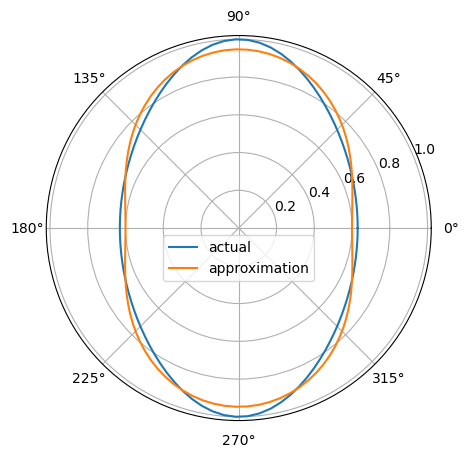
\includegraphics[width=0.5\textwidth]{images/polar_plot.png}
\caption{Polar plot of the actual function $\sqrt{ 3 \cos^2 \theta + 1} $ in blue 
and the approximated one $\frac{1}{a^2 }\cos^2 \theta + \frac{1}{b^2} \sin^2 \theta$ in orange.}
\label{fig:polarplot}
\end{figure}

Now we can express the magnitude using the Cartesian coordinates relative to the frame of the transmitter ARTVA $F_t$. 
If we consider the point $\mathbf{p}^t$\[
\mathbf{p}^t = \begin{pmatrix}
    x \\
    y \\
    z
\end{pmatrix}
\] having these coordinates $(x,y,z)$ in frame $t$, then remembering $r$ from \ref{Conversion from Cartesian to Spherical Coordinates} and $\cos\theta$ from \ref{Conversion from Spherical to Cartesian Coordinates}:
\[
\begin{cases}
r^2 = x^2 + y^2 + z^2 \\
\cos\theta = \frac{x}{r}
\end{cases}
\]

Substituting the expressions for \(r\) and \(\cos\theta\) in \ref{eq:H_mag_approx}:
\[
\left| \mathbf{H} \right| = \frac{I b^2}{4} \frac{1}{(x^2 + y^2 + z^2)^{3}} \left(\frac{1}{a^2} \frac{x^2}{x^2 + y^2 + z^2} + \frac{1}{b^2} \frac{y^2 + z^2}{x^2 + y^2 + z^2}\right)^{2/3}
\]

After simplifications and further calculations, we obtain:
\begin{equation}
    \left| \mathbf{H} \right| = \frac{m}{4 \pi} \left(\frac{(ab)^2}{b^2 x^2 + a^2 (y^2 + z^2)}\right)^{3/2}
    \label{eq:H_mag_cart}
\end{equation}
where we call $I \, \pi \, b^2$ the magnetic moment $m$.
Then, we can define $\eta$ as \cite{main}:
\[ \eta = \left( \frac{m}{4 \pi \left| \mathbf{H} \right|} \right)^{2/3} \cdot \, (ab)^2 = \]
by substituting \ref{eq:H_mag_cart}:
\[
\begin{aligned}
&= \left( \frac{m}{4 \pi \frac{m}{4 \pi} \left(\frac{(ab)^2}{b^2 x^2 + a^2 (y^2 + z^2)}\right)^{3/2}} \right)^{2/3} \cdot (ab)^2 = 
\\
&= \left( \left(\frac{b^2 x^2 + a^2 (y^2 + z^2)}{(ab)^2}\right)^{3/2}\right)^{2/3} \cdot (ab)^2
\end{aligned}
\]

So:
\begin{equation}
    \eta = b^2 x^2 + a^2 (y^2 + z^2)
    \label{eq:eta}
\end{equation}

\subsection{Finding the ARTVA position}
In order to find the victim's position $\mathbf{p}_t$ with respect to the inertial frame $F_i$, we need to use homogeneous transformations \cite{book-robotics}. 
Also from Figure \ref{fig:frames-1victim}, we can express the position of the receiver $\mathbf{p}_r$ in the inertial frame as the sum of the other two vectors:
\[
\begin{aligned}
\mathbf{p}^i &= \mathbf{p}_t^i + \mathbf{p}^t \\
\mathbf{p}^t &= R_t^i \, \mathbf{p}^t
\end{aligned}
\]
where $R_t^i$ is the rotation matrix that rotates axis $i$ to $t$ \cite{artva-gazebo}.
\begin{comment}
The matrix $R_t^i$ is the matrix which lets us express the vector in frame $i$ using the coordinates of the vector in frame $t$.Since we are expressing in the columns the coordinates of the axis of $t$ w.r.t using the axis of $i$.
Then if we have the coordinates of point $P$ with respect to frame i $\mathbf{P}$ 
(and if we know the rotation that goes from frame $i$ to frame $t$ (which also means we know the orientation and coordinates of the axis of frame $t$ with respect to those of frame $i$ $(R_t^i$ notation of Soper/this Chapman book), 
we can find the coordinates at point $P$ w.r.t frame i which is $\mathbf{P}$.
Also consider that from frame $i$ after a rotation $R_t^i$ we obtain the same orientation of frame $t$ which is just translated by the $\mathbf{P}_R$ vector.
v1 is  coordinates of the point before the translation but after the rotation, the coordinate of the point wrt the inertial frame  i are v1^i = R p^{i2}
\end{comment}

From which we can find $\mathbf{p}_t$ by multiplying by $R^T$ since $R$ is orthogonal (orthogonal $R^T = R^{-1}$):

\begin{equation}
    \mathbf{p}^t = {R_t^i}^T (\mathbf{p}_r - \mathbf{p}_t)
    \label{eq:pt}
\end{equation}

In addition, remembering how we defined the coordinates of $\mathbf{p}^t$, then from linear algebra:
\[
\begin{aligned}
x &= \mathbf{e}_x^T \mathbf{p}^t \\
y &= \mathbf{e}_y^T \mathbf{p}^t \\
x  &= \mathbf{e}_z^T \mathbf{p}^t
\end{aligned}
\]
also,
\[
x^2 = x \cdot x = \left( \mathbf{e}_x^T \mathbf{p}^t \right)^T \cdot \, \left( \mathbf{e}_x^T \mathbf{p}^t \right)
\]
and the same is valid for the other two coordinates, we will omit the calculations for the other two from now on. 
We can then substitute the expression we found for $\mathbf{p}^t$ \ref{eq:pt} and apply linear algebra properties of the transpose:
$$(ABC)^T = C^T B^T A^T$$ to calculate the transpose of $\mathbf{e}_x^T {R_t^i}^T (\mathbf{p}_r - \mathbf{p}_t)$:

\[
(\mathbf{e}_x^T {R_t^i}^T (\mathbf{p}_r - \mathbf{p}_t))^T = (\mathbf{p}_r - \mathbf{p}_t)^T {R_t^i} \mathbf{e}_x
\]
The expression for $x^2$ then becomes:
\begin{equation}
    x^2 = \left(\mathbf{p}_r - \mathbf{p}_t\right)^T {R_t^i} \mathbf{e}_x \mathbf{e}_x^T {R_t^i}^T \left(\mathbf{p}_r - \mathbf{p}_t\right)
    \label{eq:x2}
\end{equation}

Furthermore:
\[
\mathbf{e}_x \mathbf{e}_x^T =\begin{pmatrix}
1 \\
0 \\
0
\end{pmatrix}
\begin{pmatrix}
1 & 0 & 0
\end{pmatrix}
 = \text{diag}(1,0,0)
\]
and:
\[
\begin{aligned}
    \mathbf{e}_y \mathbf{e}_y^T &= \text{diag}(0,1,0) \\
    \mathbf{e}_z \mathbf{e}_z^T &= \text{diag}(0,0,1)
\end{aligned}
\]
Lastly we substitute the result found in \ref{eq:x2} in the expression of $\eta$ \ref{eq:eta}:
\[
\begin{aligned}
    \eta &=  \ b^2 \left(\mathbf{p}_r - \mathbf{p}_t\right)^T R_t^i \mathbf{e}_x \mathbf{e}_x^T {R_t^i}^T \left(\mathbf{p}_r - \mathbf{p}_t\right) + \\
    &+ a^2 \left(\mathbf{p}_r - \mathbf{p}_t\right)^T R_t^i \mathbf{e}_y \mathbf{e}_y^T {R_t^i}^T \left(\mathbf{p}_r - \mathbf{p}_t\right) +\\
    &+ a^2 \left(\mathbf{p}_r - \mathbf{p}_t\right)^T R_t^i \mathbf{e}_z \mathbf{e}_z^T {R_t^i}^T \left(\mathbf{p}_r - \mathbf{p}_t\right) =
\end{aligned}
\]
collect common terms,
\[
= \left(\mathbf{p}_r - \mathbf{p}_t\right)^T R_t^i \left( b^2 \mathbf{e}_x \mathbf{e}_x^T + a^2 \mathbf{e}_y \mathbf{e}_y^T + a^2 \mathbf{e}_z \mathbf{e}_z^T \right) {R_t^i}^T \left(\mathbf{p}_r - \mathbf{p}_t\right)=
\]
\begin{equation}
    = \left(\mathbf{p}_r - \mathbf{p}_t\right)^T R_t^i \, \text{diag}(b^2, a^2, a^2) {R_t^i}^T \left(\mathbf{p}_r - \mathbf{p}_t\right)
    \label{eq:eta2}
\end{equation}

We call the \( R_t^i \, \text{diag}(b^2, a^2, a^2) {R_t^i}^T \) matrix $M$ and the diagonal matrix $\text{diag}(b^2, a^2, a^2)$ $D$.

\subsubsection{Symmetry of \( M \)}
\textbf{Definition} \\
A matrix \( M \in \mathbb{R}^{n \times n} \) is symmetric if and only if \( M = M^T \).
\\
\textbf{Proof} \\
We compute \( M^T \):
\[
M^T = \left( R_t^i D {R_t^i}^T \right)^T = \left( {R_t^i}^T \right)^T D^T {R_t^i}^T = R_t^i D^T {R_t^i}^T
\]
Since \( D \) is a diagonal matrix, it is equal to its transpose $D^T = D$ :
$$
M^T =  R_t^i D {R_t^i}^T = M
$$

\subsubsection{Final expression for $\eta$}
By applying the distributive property to \ref{eq:eta2} and since M is symmetric:
\begin{equation}
    \eta = \mathbf{p}_r^T M \mathbf{p}_r - \mathbf{p}_r^T M \mathbf{p}_t - \mathbf{p}_t^T M \mathbf{p}_r+ \mathbf{p}_t^T M \mathbf{p}_t
    \label{eq:eta3}
\end{equation}
The vector $\mathbf{\hat{p}}_t$ gives an estimate of the true position $\mathbf{p}_t$ :
\[
\mathbf{\hat{p}}_t = M \mathbf{p}_t
\]
and since $M$ is symmetric:
\[
\mathbf{\hat{p}}_t^T =  \mathbf{p}_t^T M^T = \mathbf{p}_t^T M
\]
We substitute these expressions in \ref{eq:eta3} and use the definition of the scalar product:
\[
\eta = \mathbf{p}_r^T M \mathbf{p}_r - \mathbf{p}_r^T \mathbf{\hat{p}}_t - \mathbf{\hat{p}}_t^T \mathbf{p}_r+ \mathbf{p}_t^T M \mathbf{p}_r = \mathbf{p}_r^T M \mathbf{p}_r - 2 \mathbf{p}_r^T \mathbf{\hat{p}}_t + \mathbf{p}_t^T M \mathbf{p}_t
\]
If we define the coordinates of $\mathbf{p}_r$ :
\[
\mathbf{p}_r = \begin{pmatrix}
    x_r \\
    y_r \\
    z_r
\end{pmatrix}
\]
and
\[
M = \begin{pmatrix}
    m_{11} & m_{12} & m_{13} \\
    m_{12} & m_{22} & m_{23} \\
    m_{13} & m_{23} & m_{33} \\
\end{pmatrix}
\]
we can compute $\mathbf{p}_r^T M \mathbf{p}_r$:
\[
\mathbf{p}_r^T M \mathbf{p}_r = 
m_{11} \, x_r^2 \; + \; 2 \, m_{12} \, x_r \, y_r \; + \; 2 \, m_{13} \, z_r \, x_r \; + \;
m_{22} \, y_r^2 \; + \; 2 \, m_{23} \, y_r \, z_r \; + \; m_{33} \, z_r^2
\]
Then, we obtain a final expression for $\eta$ as in \cite{main}:
\begin{equation}
\begin{aligned}
\eta = & \ m_{11} \, x_r^2 + 2 \, m_{12} \, x_r \, y_r + 2 \, m_{13} \, z_r \, x_r \\
       & \ + m_{22} \, y_r^2 + 2 \, m_{23} \, y_r \, z_r + m_{33} \, z_r^2 \\
       & \ - 2 \, x_r \, x_t - 2 \, y_r \, y_t - 2 \, z_r \, z_t \\
       & \ + \mathbf{p}_t^T M \mathbf{p}_t
\end{aligned}
\label{eq:eta_final}
\end{equation}


\section{Multiple Victim Case}
%https://math.stackexchange.com/questions/4761965/addition-of-vectors-in-different-coordinate-systems
%https://www2.physics.ox.ac.uk/sites/default/files/2011-10-08/coordinates_pdf_51202.pdf
\begin{figure}
    \centering
    \caption{Only 2 victims case}
    \label{fig:frames-2victim}
    \tdplotsetmaincoords{70}{110}
    \begin{tikzpicture}[tdplot_main_coords]
    \draw[thick,->] (0,0,0) -- (1,0,0) node[anchor=north east]{$y_i$};
    \draw[thick,->] (0,0,0) -- (0,1,0) node[anchor=north west]{$z_i$};
    \draw[thick,->] (0,0,0) -- (0,0,1) node[anchor=south]{$x_i$};
    % Point Pt1
    \coordinate (Pt1) at (5,0,5);
    \draw[->, thick] (0,0,0) -- (Pt1) node[pos=0.5,anchor= west]{$\mathbf{p}_{t_1}$};
    % pr
    \draw[->, thick] (0,0,0) -- (p1) node[pos=0.5,anchor=west]{$\mathbf{p}_r$};
    % Point Pt2
    \coordinate (Pt2) at (0,5,3);
    \draw[->, thick] (0,0,0) -- (Pt2) node[pos=0.5,anchor= south]{$\mathbf{p}_{t_2}$};
    % Point t1p
    \coordinate (p1) at (5,5,6);
    \draw[->, thick] (5,0,5) -- (p1) node[pos=0.5, anchor=south]{$\stackrel{t_1}{\phantom{p}\bm{p}}$};      
    \node at (p1) [anchor=south] {$\bm{p}$};    
    % Point t2p
    \coordinate (p2) at (5,5,6);
    \draw[->, thick] (0,5,3) -- (p2) node[pos=0.5, anchor=south]{$\stackrel{t_2}{\phantom{p}\bm{p}}$};
    \node at (p2) [anchor=south] {$\bm{p}$};
    % Vectors H1 and H2
    \coordinate (H1) at (3,1.5,3); 
    \coordinate (H2) at (1,3,3); 
    \draw[->, thick, blue] (p1) -- (H1) node[anchor=north west]{$\mathbf{H}_1$};
    \draw[->, thick, red] (p1) -- (H2) node[anchor=north]{$\mathbf{H}_2$};
    % Angle arc
        \pic ["$\alpha$",draw = black, ->,
        angle radius=7mm,
        angle eccentricity=1.3, 
        ] { angle = H1--p1--H2};
    \coordinate (Shift) at (5,0,5);
    \tdplotsetrotatedcoordsorigin{(Shift)}
    \draw[thick,tdplot_rotated_coords,->] (0,0,0) --
    (.7,0,0) node[anchor=north]{$y_{t_1}$};
    \draw[thick,tdplot_rotated_coords,->] (0,0,0) --
    (0,.7,0) node[anchor=west]{$z_{t_1}$};
    \draw[thick,tdplot_rotated_coords,->] (0,0,0) --
    (0,0,.7) node[anchor=south]{$x_{t_1}$};
    \coordinate (Shift) at (0,5,3);
    \tdplotsetrotatedcoordsorigin{(Shift)}
    \draw[thick,tdplot_rotated_coords,->] (0,0,0) --
    (.7,0,0) node[anchor=north]{$y_{t_2}$};
    \draw[thick,tdplot_rotated_coords,->] (0,0,0) --
    (0,.7,0) node[anchor=west]{$z_{t_2}$};
    \draw[thick,tdplot_rotated_coords,->] (0,0,0) --
    (0,0,.7) node[anchor=south]{$x_{t_2}$};
    \end{tikzpicture}
\end{figure}

In the multiple victim case an ARTVA transmitter is attached to every one of the \( n \) avalanche victims, 
therefore each receiver is affected by \( n \) generated electromagnetic fields.
In Figure \ref{fig:frames-2victim}, the two victims case is represented, using the same frames as the single victim one. 
For brevity we will call \( R_1 \) and \( R_2 \) the relative orientations of frames \( t_1 \) and \( t_2 \) with respect to the reference frame \(i\).

Now, if the receiver is positioned at point \( \mathbf{p} \) in space, 
the summed effect of the electromagnetic fields can be expressed as the sum of the magnetic field intensity vector fields \(\mathbf{H}_n\):
\[
\mathbf{H}_{\text{tot}} = 
\mathbf{H}_1 + \mathbf{H}_2 + \cdots + \mathbf{H}_n
\]
For the single magnetic field intensity vector of the \(i\)-th victim, remembering \ref{eq:H_spheric}:
\[
\mathbf{H}_i = \frac{I b^2}{4\pi r^3} \left( \mathbf{e}_{r_i} \, 2 \cos \theta + \mathbf{e}_{\theta_i} \, \sin \theta \right)
\]
Furthermore, we use the same homogeneous transformations as \ref{eq:pt}:
\[
\mathbf{p}_{t_1} + R_1 \, \mathbf{p}^{t_1} = \mathbf{p}_r
\]
\[
\mathbf{p}_{t_2} + R_2 \, \mathbf{p}^{t_2} = \mathbf{p}_r
\]
which become again:
\[
\mathbf{p}^{t_1} = R_1^T \left( \mathbf{p}_R - \mathbf{p}_{t_1} \right)
\]
\[
\mathbf{p}^{t_2} = R_2^T \left( \mathbf{p}_R - \mathbf{p}_{t_2} \right)
\] 

\subsection{Total Magnitude }
Suppose the case of only two victims, the results can be then generalized.
If \( \alpha \) is the angle between the two vectors \( \mathbf{H}_1 \) and \( \mathbf{H}_2 \) on the only plane which contains both vector fields, we have:
\[
||\mathbf{H}_{\text{tot}}||^2 = ||\mathbf{H}_1||^2 + ||\mathbf{H}_2||^2 + 2 \, ||\mathbf{H}_1|| \, ||\mathbf{H}_2|| \cos \alpha
\]
Substituting the formula of the magnetic field magnitude after the approximation, with the Cartesian coordinates of reference frame $F_t$ \ref{eq:H_mag_cart}:
\[
\begin{aligned}
||\mathbf{H}_{\text{tot}}||^2 &= \left( \frac{m}{4 \pi} \right)^2 \left( \frac{(ab)^2}{b^2 \, x_1^2 + a^2 \, (y_1^2 + z_1^2)} \right)^3 
+ \left( \frac{m}{4 \pi} \right)^2 \left( \frac{(ab)^2}{b^2 \, x_2^2 + a^2 \, (y_2^2 + z_2^2)} \right)^3 + \\
& + 2 \, \cos \alpha \left( \frac{m}{4 \pi} \right)^2 \left( \frac{(ab)^2}{b^2 \, x_1^2 + a^2 \, (y_1^2 + z_1^2)} \right)^{3/2} \left( \frac{(ab)^2}{b^2 \, x_2^2 + a^2 \, (y_2^2 + z_2^2)} \right)^{3/2} = \\
&= \left( \frac{m \, (ab)^3}{4 \pi} \right)^2 \left( \left( \frac{1}{b^2 \, x_1^2 + a^2 \, (y_1^2 + z_1^2)} \right)^3 
+  \left( \frac{1}{b^2 \, x_2^2 + a^2 \, (y_2^2 + z_2^2)} \right)^3 \right. + \\
& \left. + \, 2 \, \cos \alpha \left( \frac{1}{(b^2 \, x_1^2 + a^2 \, (y_1^2 + z_1^2))(b^2 \, x_2^2 + a^2 \, (y_2^2 + z_2^2))} \right)^{3/2} \right)
\end{aligned}
\]
Note that a and b, have the same values for all the fields since they have been chosen in order to optimize the magnitude on any magnetic field intensity. 
Also we suppose that the radius $b$ and the current $I$ are the same for all the devices (so same magnetic moment $m$).

Bringing the common terms to the left side and inverting all the fractions:
\[
\begin{aligned}
\left( \frac{m \, (a b)^3}{4 \pi \, ||\mathbf{H}_{\text{tot}}||} \right)^2 &= \left( b^2 \, x_1^2 + a^2 \, (y_1^2 + z_1^2) \right)^3 + \left( b^2 \, x_2^2 + a^2 \, (y_2^2 + z_2^2) \right)^3 + \\
& + 2 \, \cos \alpha \left( (b^2 \, x_1^2 + a^2 \, (y_1^2 + z_1^2))(b^2 \, x_2^2 + a^2 \, (y_2^2 + z_2^2)) \right)^{3/2}
\end{aligned}
\]
\chapter{Control}
The purpose of this chapter is to model the dynamical system 
of each UAV and describe the control strategies used to achieve the 
desired position and velocity, while ensuring stability and robustness.
The focus of our work is to localize the position of the 
avalanche victims, therefore the control task of the drones' flight 
is limited and interested mainly in controlling the altitude 
(mantaining a fixed height) and the horizontal positions
$x$ and $y$.

Each $j$-th UAV is modeled as a quadrotor vehicle, the most common 
multirotor aerial platform, characterized by four rotors attached 
to a rigid cross-shaped airframe. Each individual rotor generates 
both a forcet and a torque. The dynamics of each quadrotor are 
described using Euler-Newton laws of motion, with the motion 
expressed in terms of both the inertial frame \( F_g \) and the 
body frame \( F_b \).
As already mentioned, we have assumed the body frame $F_b$
to coincide with the receiver frame $F_r$, relative to the
the ARTVA equipment installed on the drone; therefore 
from now on we will denote the body frame with $F_r$.

% NON MI PIACE TROPPO QUESTO PARAGRAFETTO
% Control of this underactuated system brings more challenges
% wrt to wheeled robots \cite{model_quadrotor}.
% We begin by introducing the fundamental notations and conventions, 
% followed by the complete dynamical model of the UAV. A simplification 
% is then presented, which linearizes the system and allows the use of 
% Proportional-Derivative (PD) control strategies. Finally, the control 
% strategies used to regulate the quadrotor's position and velocity are 
% detailed, including both outer-loop position control and inner-loop 
% attitude control. Lastly, a geometric control strategy is introduced 
% for application to the complete quadrotor dynamics model.

% METTERE PARAGRAFETTO DOVE SI PARLA DELLE REFERENCES USATE
% PICCOLO SOTA

\section{Notations}
We introduce the notations and conventions used in this work 
to model the quadrotor dynamics and control. 
In particular, in Table~\ref{tab:notations} we introduce and 
summarize all the quantities and variables needed.
\begin{table}[h!]
    \centering
    \begin{tabular}{lll}
        \hline
        Symbol & Description & Units \\
        \hline
        \(g\) & gravitational acceleration constant, \( g \in \mathbb{R}_{\geq 0} \) & m/s\(^2\) \\
        \(m\) & mass of the quadrotor, \( m \in \mathbb{R}_{\geq 0} \) & kg \\
        \(x_r\) & position of the quadrotor along \(x\) (east) in \(F_g\) & m \\
        \(y_r\) & position of the quadrotor along \(y\) (north) in \(F_g\) & m \\
        \(z_r\) & position of the quadrotor along \(z\) (up) in \(F_g\) & m \\
        \(v_x\) & linear velocity along \(x\) in \(F_g\) & m/s \\
        \(v_y\) & linear velocity along \(y\) in \(F_g\) & m/s \\
        \(v_z\) & linear velocity along \(z\) in \(F_g\) & m/s \\
        \(p\) & roll rate in \(F_b\) & rad/s \\
        \(q\) & pitch rate in \(F_b\) & rad/s \\
        \(r\) & yaw rate in \(F_b\) & rad/s \\
        \(\phi\) & roll angle (rotation about \(x\)-axis) & rad \\
        \(\theta\) & pitch angle (rotation about \(y\)-axis) & rad \\
        \(\psi\) & yaw angle (rotation about \(z\)-axis) & rad \\
        \(T\) & total thrust generated by the propellers, \( T \in \mathbb{R}_{\geq 0} \) & N \\
        \hline
    \end{tabular}
    \caption{Quantities used to describe the quadrotor system.}
    \label{tab:notations}
\end{table}


%DA RIVEDERE O DA TOGLIERE
The laws of motion are described in both the global inertial frame \( F_g \) 
(particularly for translational dynamics) and the body frame 
\( F_r \) (in which the rotational dynamics are expressed more 
easily). The body right-hand frame \( F_r \) is fixed to the quadrotor 
(rotates with it), with its 
origin located at the center of mass.
Its axes are defined as in \cite{model_quadrotor}:
\noindent
\begin{itemize}
    \item The \( x \)-axis points forward along the quadrotor's direction 
    of motion.
    \item The \( y \)-axis points to the left wing.
    \item The \( z \)-axis points upwards, consistent with 
    the thrust direction.
\end{itemize}
% QUI È UN BORDELLO PERCHE LA Z CHE VA IN SU 
% È PRESA DALLA CITAZIONE MENTRE LA DIREZIONE DEGLI ASSI
% VIENE DA UN ALTRA ROBA CHE FACCIO?, dovrei fare una figura io
% METTERE FOTO QUADROTOR STILIZZATO
% OPPURE COPIARE IL TKZ DELLE FRAME E METTERE QUELLA CON SOLO
% INERZIALE E RECEIVER (BODY)
\begin{figure}[h]
    \centering
    %\includegraphics[width=0.8\textwidth]{quadrotor_diagram.png}
    \caption{Quadrotor diagram showing body and inertial frames.}
    \label{fig:quadrotor_diagram}
\end{figure}

\noindent
For the inertial frame, we adopt a convention that does not use 
the standard NED\footnote{NED stands for North-East-Down.} inertial 
reference frame, to ensure consistency throughout our work. 
Instead, the inertial frame \( F_g \) follows the ENU 
\footnote{ENU stands for East-North-Up.} 
convention (Figure \ref{fig:ENU}), where the 
\( z \)-axis points upward, away from the center of the Earth. The 
inertial frame \( F_g \) is fixed to the ground, with its origin at a 
reference point (the takeoff location), and its axes are defined as:
\begin{itemize}
    \item The \( x \)-axis points east.
    \item The \( y \)-axis points north.
    \item The \( z \)-axis points opposite the gravity vector.
\end{itemize}
The ENU local tangent plane is similar to NED, except for swapping 
"down" for "up" and \( x \) for \( y \), which is more intuitive for certain 
geographical and aerial applications.

\begin{figure}[h!]
    \centering
    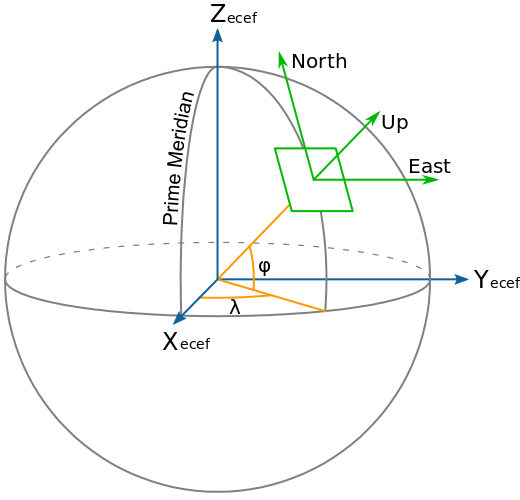
\includegraphics[width=0.5\textwidth]{images/ECEF_ENU_Longitude_Latitude_relationships.png}
    \caption[ENU and ECEF Reference Frames]{A diagram illustrating the ECEF (Earth-Centered, Earth-Fixed) 
    and ENU reference frames. 
    Adapted from a figure in \cite{ENU}.}
    \label{fig:ENU}
\end{figure}
%(IN REALTÀ È PRESA DA WIKI, VA BENE SI PUO FARE?)

\noindent
The orientation of the rigid body with respect to the inertial
frame is described by the rotation matrix 
\( \mathbf{R}^g_r(t) \in SO(3) \), which transforms vectors from the 
body frame \( F_r \) to the inertial frame \( F_g \).
The \( \mathbf{R}^g_r(t) \) rotation matrix is obtained by successive rotations around the 
inertial frame axes, these rotations define the roll, pitch and yaw angles \((\phi, \theta, \psi)\).
We specify the order of rotations as $x -y -z $:
\begin{itemize}
    \item yaw (\( \psi \)): rotation about the \(z\)-axis of the inertial frame \( F_g \).
    \item pitch (\( \theta \)): rotation about the \(y\)-axis of the inertial frame \( F_g \).
    \item roll (\( \phi \)): rotation about the \(x\)-axis of the inertial frame \( F_g \).
\end{itemize}
Since the successive rotations are relative to the fixed reference frame,
the full rotation matrix \( \mathbf{R}^g_r(t) \) is obtained as a product of the three individual rotation matrices:
\begin{align}
\mathbf{R}^g_r & = 
\mathbf{R}_z(\psi) \mathbf{R}_y(\theta) \mathbf{R}_x(\phi) \nonumber\\
& =
\begin{bmatrix}
\cos\psi & -\sin\psi & 0 \\
\sin\psi & \cos\psi & 0 \\
0 & 0 & 1
\end{bmatrix}
\begin{bmatrix}
\cos\theta & 0 & \sin\theta \\
0 & 1 & 0 \\
-\sin\theta & 0 & \cos\theta
\end{bmatrix}
\begin{bmatrix}
1 & 0 & 0 \\
0 & \cos\phi & -\sin\phi \\
0 & \sin\phi & \cos\phi
\end{bmatrix} \nonumber\\ 
& =
\resizebox{0.84\textwidth}{!}{$
\begin{bmatrix}
\cos\psi \cos\theta & \cos\psi \sin\theta \sin\phi - \sin\psi \cos\phi & \cos\psi \sin\theta \cos\phi + \sin\psi \sin\phi \\
\sin\psi \cos\theta & \sin\psi \sin\theta \sin\phi + \cos\psi \cos\phi & \sin\psi \sin\theta \cos\phi - \cos\psi \sin\phi \\
-\sin\theta & \cos\theta \sin\phi & \cos\theta \cos\phi
\end{bmatrix}
$}
\label{eq:attitude}
\end{align}
    
    
\noindent
\textbf{Note}
\\
Considering \( \mathbf{x} \in \mathbb{R}^3 \), we define a square matrix to 
be skew-symmetric \( \mathbf{S}(\mathbf{x}) \in \mathfrak{so}(3) \)
if and only if:
\begin{equation}
\mathbf{S}(\mathbf{x})\mkern-3mu^\top \mkern-4mu + \mathbf{S}(\mathbf{x}) = 0
\label{eq:skew_symmetric_condition}
\end{equation}
\noindent
Any rotation matrix \( \mathbf{R}(t) \in SO(3)\) satisfies the orthogonality condition:
\begin{equation}
\mathbf{R}(t) \, \mathbf{R}\mkern-3mu^\top\mkern-4mu(t) = \mathbf{I}
\label{eq:orthogonality_condition}
\end{equation}
\noindent
Computing the time derivative on both sides of \eqref{eq:orthogonality_condition} gives:
\begin{equation}
\dot{\mathbf{R}}(t) \, \mathbf{R}\mkern-3mu^\top\mkern-4mu(t) + \mathbf{R}(t) \, \dot{\mathbf{R}}\mkern-3mu^\top\mkern-4mu(t) = 0
\label{eq:time_derivative_orthogonality}
\end{equation}
\noindent
This is the skew-symmetry condition \eqref{eq:skew_symmetric_condition} 
for a matrix defined as:
\begin{equation}
\mathbf{S}(t) \stackrel{\Delta}{=} \dot{\mathbf{R}}(t) \, \mathbf{R}(t)\mkern-3mu^\top
\label{eq:def_skew_symmetric}
\end{equation}
\noindent
By postmultiplying $\mathbf{R}(t)$ on both sides of \ref{eq:def_skew_symmetric} we
obtain an expression for the variation in time of any rotation matrix:
\begin{equation}
\dot{\mathbf{R}}(t) = \mathbf{S}(t) \, \mathbf{R}(t)
\label{eq:skew_symmetric_rotation}
\end{equation}
\noindent
Since $\mathbf{R}(t)$ is the product of basic rotations with respect to the fixed frame and  
denoting with $ \boldsymbol{\omega}(t) = (\omega_x, \omega_y,  \omega_z)^\top \in \mathbb{R}^3$ the angular velocity of the body frame with respect to the fixed frame, 
we can repeat the same process to find an expression of $\mathbf{S}$ which depends on the time
derivative of the orientation angles, \cite{book-robotics}:
\begin{equation}
\mathbf{S}(\boldsymbol{\omega}) = 
\begin{bmatrix}
    0 & -\omega_z & \omega_y \\
    \omega_z & 0 & -\omega_x \\
    -\omega_y & \omega_x & 0
\end{bmatrix}
\label{eq:skew_symmetric_matrix}
\end{equation}
\noindent
Furthermore, the angular velocity of the rotating body frame with respect to the fixed frame is related with the angular velocity
expressed in the receiver frame as:
\begin{equation}
     \boldsymbol{\omega} = \mathbf{R}^g_r \, {}^r\mkern-3mu\boldsymbol{\omega}
    \label{eq:angular_velocity_inertial}
\end{equation}
\noindent
Then, we substitute Eq.\ref{eq:angular_velocity_inertial} in Eq.\ref{eq:def_skew_symmetric} to obtain the 
the skew-symmetric matrix of ${}^r \boldsymbol{\omega}$, in the body frame:
\begin{equation}
    \mathbf{S}(\boldsymbol{\omega}) =  \mathbf{S}(\mathbf{R}^g_r \, {}^r\mkern-3mu\boldsymbol{\omega}) 
    \label{eq:S_body}
\end{equation}
\noindent
Using the properties of skew-symmetric matrices:
\begin{equation}
    \mathbf{S}(\mathbf{R}^g_r \, {}^r\mkern-3mu\boldsymbol{\omega}) = \mathbf{R}^g_r \, \mathbf{S}({}^r\mkern-3mu\boldsymbol{\omega}) \, {\mathbf{R}^g_r}^\top 
    \label{eq:skew_symm_property}
\end{equation}
Substituting this result \eqref{eq:skew_symm_property} in Eq.\ref{eq:skew_symmetric_rotation}:
\begin{equation}
    \dot{\mathbf{R}^g_r} = \mathbf{R}^g_r \, \mathbf{S}({}^r\mkern-3mu\boldsymbol{\omega}) \, {\mathbf{R}^g_r}\mkern-3mu^\top  \, \mathbf{R}^g_r = \mathbf{R}^g_r \, \mathbf{S}({}^r\mkern-3mu\boldsymbol{\omega})
    \label{eq:skew_symmetric_body}
\end{equation}
We obtain the same expression of the inertial frame in the body frame.

\section{Complete Quadrotor Dynamics}
\subsection{Translational Dynamics}
Since the position of the UAV's center of gravity is represented by \( \mathbf{p}_r \in \mathbb{R}^3 \), 
expressed in the inertial frame \( F_g \), we denote its time derivative as \( \dot{\mathbf{p}}_r \) and 
the linear acceleration as \( \ddot{\mathbf{p}}_r \).
%%%%%%%%%%%%%% QUI C E COME CI SI ARRIVA
% Applying Newton's second law in the body frame, the translational dynamics are expressed as:
% \[
% m \frac{\mathrm{d}}{\mathrm{d}t}\mathbf{v}^b = \mathbf{f}^b,
% \]
% where:
% \begin{itemize}
%     \item \(\mathbf{v}^b = [v_x^b, v_y^b, v_z^b]^\top\): Linear velocity in the body frame.
%     \item \(\mathbf{f}^b\): Total force acting on the quadrotor, including thrust, drag, and gravity.
% \end{itemize}
% In the inertial frame, the translational dynamics of the quadrotor are given by:
% \[
% m \ddot{\mathbf{p}} = \mathbf{R}^\top \mathbf{f}^b - m g \mathbf{e}_z,
% \]
% where:
% \begin{itemize}
%     \item \(\ddot{\mathbf{p}}\): Acceleration of the quadrotor in the inertial frame.
%     \item \(\mathbf{e}_z = [0, 0, 1]^\top\): Unit vector in the \(z\)-direction of the inertial frame.
%     \item \(\mathbf{f}^b = [0, 0, f_{\text{thrust}}]^\top\): Force vector due to thrust in the body frame.
% \end{itemize}
% By transforming gravity into the body frame, we write:
% \[
% \mathbf{f}^b = \mathbf{R} \mathbf{f}^i,
% \]
% where \(\mathbf{f}^i\) includes gravitational and aerodynamic forces expressed in the inertial frame.


Then, by applying Newton-Euler first law, we obtain the 
translational dynamics of the quadrotor in the fixed inertial frame $F_g$ as in \cite{simplified_model}:
\begin{equation}
M \ddot{\mathbf{p}}_r = \sum \mathbf{F}_{\text{ext}} 
= T \, \mathbf{R}_r^g \, \mathbf{e}_z - M g \, \mathbf{e}_z - \mathbf{d}_f
\label{eq:translational_dyn}
\end{equation}
where \( \mathbf{F}_{\text{ext}} \) denotes all the external forces acting on the vehicle, which
includes the thrust force \( T \in \mathbb{R}_{\geq 0} \) generated by the propellers and therefore  
represents the control force, the input of the system which can be controlled.
It is aligned with the body \( z \)-axis by construction, as it is the sum of the single
forces generated by the aligned rotors. 
It also includes the gravitational force \( M g \), which instead is always directed towards the center of 
the Earth and therefore negative in our ENU fixed reference system. 
Finally, \( \mathbf{d}_f \) represents the disturbance forces, accounting for exogenous effects such as 
aerodynamic drag and wind disturbances \cite{control_quadrotor_main}.


\subsection{Rotational Dynamics} 
Newton-Euler's second law describes the variation in time of the angular momentum of a rigid body $\mathbf{L}$ 
in terms of the inertial reference frame, \cite{quadrotor_modeling_control_book}, \cite{book-robotics}:
\begin{equation}
    \frac{\mathrm{d} \mathbf{L}}{\mathrm{d}t} = \sum \boldsymbol{\tau}_{\text{ext}}
    \label{eq:NE-2}
\end{equation}
where \( \mathbf{L} \in \mathbb{R}^3 \) is the angular momentum of the rigid body,
expressed in the fixed inertial frame \( F_g \), and \( \boldsymbol{\tau}_{\text{ext}} \in \mathbb{R}^3 \) 
represents the total applied torque about the center of mass, which includes contributions 
from the control inputs, external disturbances, and aerodynamic effects.
\noindent \\
The angular momentum \( \mathbf{L} \) is related to the angular velocity as:
\begin{equation}
    \mathbf{L} = \mathbf{J} \, \boldsymbol{\omega}
    \label{eq:angular_momentum}
\end{equation}
where \( \mathbf{J} \in \mathbb{R}^{3 \times 3} \) is the inertia matrix of the rigid body, 
which is symmetric and positive definite (\( \mathbf{J} = \mathbf{J}^\top > 0 \)).
\noindent \\
However, it is more convenient to express the rotational dynamics 
in the body frame \( F_r \) of the rigid body, since the inertia matrix remains constant in this case. 
The opposite is not true, in fact the inertia matrix in the inertial frame is given by:
\begin{equation}
    \mathbf{J} =  \mathbf{R}^g_r \, {}^r\mkern-3mu\mathbf{J} \,  {\mathbf{R}^g_r}\mkern-2mu^\top 
    \label{eq:inertia_rot}
\end{equation}
Therefore, we substitute this property of the inertia matrix \eqref{eq:inertia_rot} and 
Eq.\ref{eq:angular_velocity_inertial} in Eq.\ref{eq:NE-2}, 
and use the result obtained earlier in \ref{eq:skew_symmetric_body}:
\begin{align}
    \frac{\mathrm{d} (\mathbf{J} \boldsymbol{\omega})}{\mathrm{d}t} &= 
    \dot{\mathbf{R}}^g_r \, {}^r\mkern-3mu\mathbf{J} \, {\mathbf{R}^g_r}\mkern-2mu^\top  {}^r\mkern-2mu\boldsymbol{\omega} +
    \mathbf{R}^g_r \, {}^r\mkern-3mu\mathbf{J} \, \dot{\mathbf{R}^g_r}\mkern-2mu^\top  {}^r\mkern-2mu\boldsymbol{\omega} \notag 
     + \mathbf{R}^g_r \, {}^r\mkern-3mu\mathbf{J} \, {\mathbf{R}^g_r}\mkern-2mu^\top  {}^r\mkern-2mu\dot{\boldsymbol{\omega}} \notag \\
    &= {}^r\mkern-3mu\mathbf{J} \, {}^r\dot{\boldsymbol{\omega}} + 
    {}^r\mkern-2mu\boldsymbol{\omega} \times ({}^r\mkern-3mu\mathbf{J} \, {}^r\mkern-2mu\dot{\boldsymbol{\omega}})
    \label{eq:derivazione_rotational_law}
\end{align}
\noindent\\
In the end, by comparing the right side of Eq.~\eqref{eq:derivazione_rotational_law}
with the right side of Eq.\ref{eq:NE-2}, we obtain as in \cite{control_quadrotor_main}
the complete rotational motion of the rigid body:
\begin{equation}
    {}^r\mkern-3mu\mathbf{J} \, {}^r\dot{\boldsymbol{\omega}} +
    {}^r\mkern-2mu\boldsymbol{\omega} \times ({}^r\mkern-3mu\mathbf{J} \, {}^r\mkern-2mu\dot{\boldsymbol{\omega}})
     = \sum \boldsymbol{\tau}_{\text{ext}}
    \label{eq:rot_dyn_final}
\end{equation}

\noindent\\
The inertia matrix \( {}^r\mkern-3mu\mathbf{J} \) depends on the geometry and mass distribution of the rigid body. 
For the quadrotor, assuming a rigid body structure with a dense spherical core of mass \( M \) and radius \( r \), 
along with four point masses \( m \) located at a distance \( l \) from the center, 
the inertia matrix takes the diagonal form:
\[
{}^r\mkern-3mu\mathbf{J} = 
\begin{bmatrix}
J_x & 0 & 0 \\
0 & J_y & 0 \\
0 & 0 & J_z
\end{bmatrix},
\]
where:
\[
J_x = J_y = \frac{2}{5} M r^2 + 2 l^2 m, \quad J_z = \frac{2}{5} M r^2 + 4 l^2 m.
\]
\noindent
Substituting Eq.~\eqref{eq:angular_momentum} into Eq.~\eqref{eq:rot_dyn_final}, we obtain the 
rotational dynamics law:
\begin{equation}
    {}^r\mkern-3mu\mathbf{J} \, {}^r\mkern-4mu\dot{\boldsymbol{\omega}} + {}^r\mkern-4mu\boldsymbol{\omega} \times 
    ({}^r\mkern-3mu\mathbf{J} \, {}^r\mkern-4mu\boldsymbol{\omega}) = \boldsymbol{\tau}_{\text{u}} + \mathbf{d}_{\tau}
    \label{eq:rotational_dynamics}
\end{equation}
where $\boldsymbol{\tau}_{\text{u}} \in \mathbb{R}^3$ is the controlled input
torque vector dependent on the single torque generated
by each rotor and with $\mathbf{d}_{\tau}$ we denote 
all the external disturbances.

\noindent\\
In addition, we need to relate the angular velocity \( {}^r\mkern-4mu\boldsymbol{\omega} \) in the body frame 
to the time derivatives of the roll, pitch and yaw angles (\( \phi, \theta, \psi \)) 
in the inertial frame. We assume that the variation of the angles  $\dot{\phi}, \dot{\theta}, \dot{\psi}$
is small and therefore $\dot{\mathbf{R}}_x(\phi) = \dot{\mathbf{R}}_x(\theta) =  \dot{\mathbf{R}}_x(\psi) = \mathbf{I}$:
\begin{equation}
    {}^r\boldsymbol{\omega} = 
    \begin{pmatrix}
        p \\ q \\ r
    \end{pmatrix}
    =
    \begin{pmatrix}
        1 & 0 & -\sin\theta \\
        0 & \cos\phi & \sin\phi\cos\theta \\
        0 & -\sin\phi & \cos\phi\cos\theta
    \end{pmatrix}
    \begin{pmatrix}
        \dot{\phi} \\ \dot{\theta} \\ \dot{\psi}
    \end{pmatrix}
    \label{eq:angular_rates_to_rpy}
\end{equation}

\noindent\\
Finally, also the rotation matrix \( \mathbf{R}_r^g (t) \) 
evolves in time as the rigid body rotates in space, following the result obtained earlier
in Eq.\ref{eq:skew_symmetric_body}:
\begin{equation}
    \dot{\mathbf{R}}_r^g = \mathbf{R}_r^g \, \mathbf{S}({}^r\boldsymbol{\omega})
    \label{eq:rotation_matrix_dynamics_final}
\end{equation}
where \( \mathbf{S}({}^r\mkern-4mu\boldsymbol{\omega}) \) is a skew-symmetric matrix
in the form of \eqref{eq:skew_symmetric_matrix}, but relative to the body frame components:
\begin{equation}
    \mathbf{S}({}^r\mkern-3mu\mathbf\boldsymbol{\omega}) = 
    \begin{bmatrix}
        0 & -r & q \\
        r & 0 & -p \\
        -q & p & 0
    \end{bmatrix}
\label{eq:skew_symmetric_matrix_body}
\end{equation}

\subsection{Final Complete Quadrotor Dynamics}
Combining the translational and rotational dynamics, the complete UAV dynamics is given by the system of equations
\ref{eq:translational_dyn}, \ref{eq:rotation_matrix_dynamics_final} and \ref{eq:rotational_dynamics}:
\begin{equation}
\begin{cases}
    M \ddot{\mathbf{p}}_r = T \, \mathbf{R}_r^g \, \mathbf{e}_z - M g \, \mathbf{e}_z - \mathbf{d}_f \\[6pt]
    \dot{\mathbf{R}}_r^g = \mathbf{R}_r^g \, \mathbf{S}({}^r\mkern-4mu\boldsymbol{\omega}) \\[6pt]
    {}^r\mkern-4mu\mathbf{J} \, {}^r\mkern-4mu\dot{\boldsymbol{\omega}} = 
    - {}^r\mkern-4mu\boldsymbol{\omega} \times 
    ({}^r\mkern-4mu\mathbf{J} \, {}^r\mkern-4mu\boldsymbol{\omega}) + \boldsymbol{\tau}_{\text{u}} + \mathbf{d}_{\tau}   
\end{cases}
\label{eq:final_model}
\end{equation}
More explicitly we can expand these equations and thanks to inverting Eq.\ref{eq:angular_rates_to_rpy}
and how we defined rotation matrix $\mathbf{R}_r^g$ in Eq.\ref{eq:attitude}, we obtain
a system with twelve states and four control inputs:
{\large
\begin{equation}
    \begin{cases}
        \dot{x}_r = v_x \\[6pt]
        \dot{y}_r = v_y \\[6pt]
        \dot{z}_r = v_z \\[6pt]
        \dot{v_x} = -d_{f,x} + (\cos(\psi) \sin(\theta) \cos(\phi) + \sin(\psi) \sin(\phi)) \frac{T}{M} \\[6pt]
        \dot{v_y} = -d_{f,y} + (\sin(\psi) \sin(\theta) \cos(\phi) - \cos(\psi) \sin(\phi)) \frac{T}{M} \\[6pt]
        \dot{v_z} = -d_{f,z} - g + \cos(\theta) \cos(\phi) \frac{T}{M} \\[6pt]
        \dot{\phi} = p + \sin(\phi) \tan(\theta) q + \cos(\phi) \tan(\theta) r \\[6pt]
        \dot{\theta} = \cos(\phi) q - \sin(\phi) r \\[6pt]
        \dot{\psi} = \sin(\phi) \sec(\theta) q + \cos(\phi) \sec(\theta) r \\[6pt]
        \dot{p} = \tau_{\phi} + \frac{I_y - I_z}{I_x} qr + \frac{\tau_\phi}{I_x} \\[8pt]
        \dot{q} = \tau_{\theta} + \frac{I_z - I_x}{I_y} pr + \frac{\tau_\theta}{I_y} \\[8pt]
        \dot{r} = \tau_{\psi} + \frac{I_x - I_y}{I_z} pq + \frac{\tau_\psi}{I_z}
    \end{cases}
    \label{eq:final_model_more}
\end{equation}}
\noindent
where $\tau_{\phi}, \tau_{\theta}, \tau_{\psi}$  are the components of input
torque vector $\boldsymbol{\tau}_{\text{u}} = (\tau_{\phi}, \tau_{\theta}, \tau_{\psi})^\top $.
\noindent
\\
In a compact state-space form:
\begin{equation}
    \dot{\boldsymbol{\xi}} = f(\boldsymbol{\xi}) + g(\boldsymbol{\xi}) \boldsymbol{u}
\end{equation}
where:
\[
\boldsymbol{\xi} = [x_r, y_r, z_r, v_x, v_y, v_z, \phi, \theta, \psi, p, q, r]^\top
\]
\[
\boldsymbol{u} = [T, \tau_\phi, \tau_\theta, \tau_\psi]^\top
\]
The non-linear dynamics of the state is desbribe by \( f(\boldsymbol{\xi}) \), 
while \( g(\boldsymbol{\xi}) \) represents the control input relationships
with the system.


\section{Simplified Dynamics}
To facilitate control design, we consider a simplified model of the quadrotor dynamics,
as proposed in \cite{simplified_model}. 
This model assumes nominal conditions with no external 
disturbances and employs a small angle approximation 
for the roll (\( \phi \)) and pitch (\( \theta \)) angles. 
Additionally, we assume symmetric mass distribution 
and negligible aerodynamic and gyroscopic effects.
\noindent
Under these assumptions:
\begin{itemize}
    \item Small angular velocities and small angles allow \( (\dot{\phi}, \dot{\theta}, \dot{\psi}) \approx (p, q, r) \),
     simplifying the rotational dynamics.
    \item The Coriolis or gyroscopic term  \( {}^r\boldsymbol{\omega} \times (\mathbf{J} \, {}^r\boldsymbol{\omega}) \) 
    in the rotational dynamics is negligible for stabilization tasks, where angular velocities remain small.
\end{itemize}
The simplified dynamics are:
\begin{equation}
\begin{cases}
    M \ddot{\mathbf{p}}_r = T \, \mathbf{R}_r^g \, \mathbf{e}_z - M g \, \mathbf{e}_z \\[6pt]
    \mathbf{J} \, {}^r\mkern-4mu\dot{\boldsymbol{\omega}} = \boldsymbol{\tau}_{\text{u}}
\end{cases}
\label{eq:simplified_rotational_dynamics}
\end{equation}
Explicitly expanded as:
\begin{subequations}
\begin{align}
    \ddot{x}_r &= (\cos\psi \sin\theta \cos\phi + \sin\psi \sin\phi) \frac{T}{M} \label{eq:position_control_x}\\[6pt] 
    \ddot{y}_r &= (\sin\psi \sin\theta \cos\phi - \cos\psi \sin\phi) \frac{T}{M} \label{eq:position_control_y}\\[6pt] 
    \ddot{z}_r &= \cos\theta \cos\phi \frac{T}{M} - g  \label{eq:position_control_z}\\[6pt] 
    \dot{\phi} &= \frac{\tau_{\phi}}{I_x} \\[8pt]
    \dot{\theta} &= \frac{\tau_{\theta}}{I_y} \\[8pt]
    \dot{\psi} &= \frac{\tau_{\psi}}{I_z}
\end{align}
\label{eq:simplified_model}
\end{subequations}
This simplified model reduces the complexity of the quadrotor dynamics,
making it adapt to be controlled by simple control strategies such as 
PID\footnote{PID stands for Proportional-Integral-Derivative} control.

\section{PD Control}
\label{sec:PID_control}
In this section, we implement a PID controller 
based on the simplified model from Section~\ref{eq:simplified_model},
but we aslo apply it to the full quadrotor dynamics described in Eqs.\ref{eq:final_model_more},
to evaluate its effectiveness in a real world scenario.

The primal objective is to regulate the altitude $z$ and the 
horizontal positions \( x \) and \( y \) of the quadrotor along a 
specified trajectory $\mathbf{x}_d(t) \in \mathbb{R}^3$.
In order to do so we define position error $\mathbf{e}(t) \in \mathbb{R}^3$
between the actual position $p_r(t)$ f the $j$-th UAV and the desired trajectory as:
\[
    \mathbf{e}(t) = \mathbf{x}_d(t) - \mathbf{p}_r(t) = 
    \begin{bmatrix}
        e_x(t) \\
        e_y(t) \\
        e_z(t)
    \end{bmatrix} =
    \begin{bmatrix}
        x_d(t) - p_{r_x}(t) \\
        y_d(t) - p_{r_y}(t) \\
        z_d(t) - p_{r_z}(t)
    \end{bmatrix}
\]
In Figure\ref{fig:control_traj_tracking}, we define the block
diagram which shows the hierarchical PID control of the full 
quadrotor dynamics.

\subsection{Position Control}
Focusing firstly on the altitude $z$,
we drive the error esponentially to zero by controlling the acceleration
vector of the quadrotors $\ddot{z}_r$ as in \cite{simplified_model} to satisfy:
\[
 K_{p_z} ( z_r - z_d )  + K_{d_z} (\dot{z}_r - \dot{z}_d ) + \ddot{z}_r - \ddot{z}_d = 0
\]
\noindent
Therefore, the virtual input of our control system is:
\begin{equation}
    \ddot{z}_r  =  K_{p_z} e_z + K_{d_z} \dot{e}_z + \ddot{z}_d
    \label{eq:virtual_input}
\end{equation}
where \( K_{p_z} \) and \( K_{d_z} \) are the  proportional and derivative gains, respectively.

\noindent
From the simplified dynamics \eqref{eq:position_control_z}, 
the control thrust \( T \) required to maintain the altitude is given by:
\begin{equation}
    T = \frac{M}{\cos\theta \cos\phi} \, (g + \ddot{z}_r)
    \label{eq:true_input}
\end{equation}
\noindent
Substituting \( \ddot{z}_r \) from Eq.\ref{eq:virtual_input} in Eq.\ref{eq:true_input},
we obtain:
\begin{equation}
    T = \frac{M}{\cos\theta \cos\phi} \, \left( g + K_{p_z} e_z + K_{d_z} \dot{e}_z + \ddot{z}_d \right)
    \label{eq:desired_thrust}
\end{equation}
%Since we do not need any vertical acceleration we specify $\ddot{z}_d = 0$, questo dillo nell implementazione.
%nell implementazione dire che la traiettoria scelat è una TRAIETTORIA ESPONENZIALE 

\begin{figure}
    \resizebox{\textwidth}{!}{
    \centering
    \begin{tikzpicture}[font=\sffamily, thick, node distance=2cm]
        % Nodes
        \node[draw, fill=orange!50, text centered, minimum width=3cm, minimum height=1.5cm] (attitude) {Attitude Control};
        \node[draw, fill=ocra!50, text centered, minimum width=3cm, minimum height=1.5cm, 
        below right=1cm and -0.25cm of attitude] (position) {Position Control};
        \node[draw=black, line width=2pt, inner sep=0pt, anchor=center, minimum width=3cm, minimum height=2.5cm] 
        at ($(attitude) + (8cm, -0.25cm)$) (drone) {
        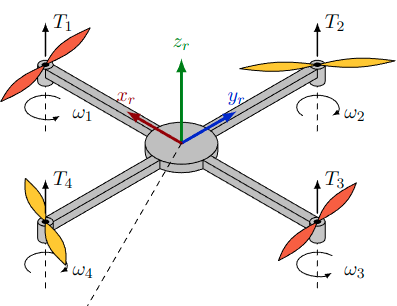
\includegraphics[height=2.5cm, width=3cm]{images/quad_model.png}};
        % Arrows
        % Attitude to Drone
        \draw[-stealth] (attitude.east) -- ([yshift=0.25cm] drone.west) 
            node[midway, above] {$\tau_\varphi, \tau_\vartheta, \tau_\psi$};
        % Position to Attitude
        \draw[-stealth] (position.west) -| (attitude.south) 
            node[near end, left] {$\varphi_d, \vartheta_d, \psi_d$};
        % Feedback loop from Drone to Attitude
        \draw[-stealth] ([xshift=1cm] drone.east) 
        -- ++(0,1.5cm) % Move up by 1 unit (cm by default in TikZ)
        -- ([yshift=0.5cm] attitude.north) % Move left towards attitude.north with a shift
        -- (attitude.north); % Move down to the exact attitude.north position
        % Incorrect arrow corrected: Drone east side to itself
        \draw (drone.east) -- ++(1cm, 0)
        node[right] {$\mathbf{e}$};
        % Feedback loop from Drone to Position
        \draw[-stealth] ([xshift=1cm] drone.east) |- ([yshift=0.25cm]position.east);
        % Position to Drone (Thrust, shifted down)
        \draw[-stealth] (position.north) |- ([yshift=-0.25cm] drone.west) 
            node[midway, below right] {$T$};
        % Position Control Outputs to its East Side
        \draw[-stealth] ([xshift=3cm, yshift=-0.25cm] position.east) -- ([yshift=-0.25cm] position.east)
            node[midway, below] {$\mathbf{x}_d, \mathbf{v}_d, \mathbf{a}_d$};    
    \end{tikzpicture}}
    \caption{Block diagram of the PID control for trajectory tracking}
    \label{fig:control_traj_tracking}
\end{figure}

The control strategy we have adopted is hierarchical \cite{model_quadrotor}
since we have given priority to the 
altitude and horizontal positions control to determine the desired input thrust;
only after we determine this quantity
we define in cascade the control torques $\tau\theta, \tau\phi, \tau\psi$.

As before we want the position error to esponentially converge to zero,
therefore we desire:
\begin{equation}
    \begin{cases}
        K_{p_x} ( x_r - x_d )  + K_{d_x} (\dot{x}_r -\dot{x}_d) + \ddot{x}_r -\ddot{x}_d  = 0 \\[6pt]
        K_{p_y} (y_r - y_d )  + K_{d_y} ( \dot{y}_r - \dot{y}_d) +  \ddot{y}_r - \ddot{y}_d = 0
    \end{cases}
\end{equation}
where $K_{p_x}$ and $K_{p_y}$ are proportional gains, and $K_{d_x}$ and $K_{d_y}$ are derivative gains.
\noindent \\
From the simplified translational dynamics, Equations \ref{eq:position_control_x}
and \ref{eq:position_control_y}, we find the desired pitch \( \theta_d \) 
and roll \( \phi_d \) angles that ensure the system converges to the desired trajectory.
We substitute the desired angles and obtain:
\begin{subequations}
    \begin{align}
    \frac{M}{T} \ddot{x}_r &= \cos\psi \sin\theta \cos\phi + \sin\psi \sin\phi \label{eq:T_x} \\[6pt]
    \frac{M}{T} \ddot{y}_r &= \sin\psi \sin\theta \cos\phi - \cos\psi \sin\phi \label{eq:T_y}
    \end{align}
\end{subequations}
\subsection{Attitude Control}
\noindent
After performing algebraic and trigonometric manipulations, we derive expressions for the desired roll and pitch angles:
\begin{equation}
    \phi_d =  \arcsin\left(  (T_y \cos\psi - T_x \sin\psi) \right)
    \label{eq:desire_phi}
\end{equation}
\begin{equation}
    \theta_d = - \arcsin\left(\frac{T_x \cos\psi + T_y \sin\psi}{ \cos\phi_d } \right)
    \label{eq:desire_theta}
\end{equation}
where $T_x = \frac{M}{T} \ddot{x}_r$ and $T_y = \frac{M}{T} \ddot{y}_r$ are the
desired components of the thrust vector in $x$ and $y$ and are found
using Equations \ref{eq:T_x} and \ref{eq:T_y} respectively.

\noindent\\
For the desired yaw angle, we use the relationship between the velocity 
components, so that the quadrotor mantains the correct heading direction.
Specifically, the yaw angle is determined as:
\begin{equation}
    \psi_d = \arctan2(\dot{y}_d, \dot{x}_d),
\end{equation}

\noindent
Using the desired angles $\phi_d$, $\theta_d, \psi_d$, the control torques are defined as:
\begin{equation}
    \label{eq:input_phi}
    \tau_\phi = I_x \left(  K_{p_\phi} e_\phi + K_{d_\phi} \dot{e}_\phi \right)
\end{equation}
\begin{equation}
    \label{eq:input_theta}
    \tau_\theta = I_y \left(K_{p_\theta} e_\theta + K_{d_\theta} \dot{e}_\theta \right)
\end{equation}
\begin{equation}
    \label{eq:input_psi}
    \tau_\psi = I_z \left(K_{p_\psi} e_\psi + K_{d_\psi} \dot{e}_\psi \right)
\end{equation}
Where $K_{p_\phi}$, $K_{d_\phi}$, $K_{p_\theta}$, $K_{d_\theta}$, $K_{p_\psi}$, and $K_{d_\psi}$ 
represent the proportional and derivative gains for roll, pitch, and yaw, respectively. 
While the input force was defined earlier in Eq.\ref{eq:true_input}.

\subsection{Rotor Velocities}
\tikzset
{%
  pics/cylinder/.style n args={3}{% #1 = radius, #2 = height, #3 = angle
    code={%
      \draw[pic actions] (135:#1) arc (135:315:#1) --++ (0,0,#2) arc (315:135:#1) -- cycle;
      \draw[pic actions] (0,0,#2) circle (#1);
      \foreach\z in {0,1}
      {
        \begin{scope}[canvas is xy plane at z=\z*\h]
          \coordinate (-cen\z) at       (0,0);
          \coordinate (-ESE\z) at    (-#3:#1);
          \coordinate (-ENE\z) at     (#3:#1);
          \coordinate (-NNE\z) at  (90-#3:#1);
          \coordinate (-NNW\z) at  (90+#3:#1);
          \coordinate (-WNW\z) at (180-#3:#1);
          \coordinate (-WSW\z) at (180+#3:#1);
          \coordinate (-SSW\z) at (270-#3:#1);
          \coordinate (-SSE\z) at (270+#3:#1);
        \end{scope}
      }
    }},
}
\begin{figure}
    \centering
    \begin{tikzpicture}[isometric view,line cap=round,line join=round]
    % dimensions
    \def\l{3.7}    % boom length
    \def\R{0.7}    % body radius
    \def\r{0.15} % motor radius
    \def\h{0.2}  % boom and body height
    \pgfmathsetmacro\A{asin(\r*sin(45)/\R)}
    % paths to situate the coordinates
    \foreach[count=\i]\j in {E,N,W,S}
      \pic[draw=none] (\j) at (90*\i-90:\l) {cylinder={\r}{\h}{45}};
    \pic[draw=none] (O) {cylinder={\R}{\h}{\A}};
    % rotations
    \foreach \i/\j in {1/1, 2/-1, 3/1, 4/-1}
    {
      \draw[dashed] (90*\i:\l) + (0,0,-\h) --++ (0,0,-7*\h);
      \begin{scope}[shift={(180-90*\i:\l)},canvas is xy plane at z=-4*\h,x=\j cm]
        \draw[-latex] (.4,0) arc (0:270:0.4) node [right, xshift=1mm] {$\omega_\i$};
      \end{scope}
    }
    % motors
    \foreach\i in {E,N,W,S}
      \pic[fill=gray!90,shift={(0,0,-\h)}] at (\i-cen0) {cylinder={\r}{2*\h}{45}};
    % boom, east
    \draw[fill=gray] (E-SSW1) arc (225:135:\r) -- (O-ENE1) arc (\A:-\A:\R) -- cycle;
    \draw[fill=gray] (E-SSW1) -- (E-SSW0) -- (O-ESE0) -- (O-ESE1) -- cycle;
    % boom, north
    \draw[fill=gray] (N-SSE1) arc (315:225:\r) -- (O-NNW1) arc (90+\A:90-\A:\R) -- cycle;
    \draw[fill=gray] (N-SSW1) -- (N-SSW0) -- (O-NNW0) -- (O-NNW1) -- cycle;
    % frame
    \pic[fill=gray] {cylinder={\R}{\h}{\A}};
    % boom, west
    \draw[fill=gray] (W-NNE1) arc (45:-45:\r) -- (O-WSW1) arc (180+\A:180-\A:\R) -- cycle;
    \draw[fill=gray] (W-SSE1) -- (W-SSE0) -- (O-WSW0) -- (O-WSW1) -- cycle;
    % boom, south
    \draw[fill=gray] (S-NNW1) arc (135:45:\r) -- (O-SSE1) arc (270+\A:270-\A:\R) -- cycle;
    \draw[fill=gray] (S-NNW1) -- (S-NNW0) -- (O-SSW0) -- (O-SSW1) -- cycle;
    % Propellers with alternating red and yellow colors
    \foreach[count=\i]\j in {140,10,60,15}
    {
      \begin{scope}[shift={(90*\i-90:\l)},rotate around z=\j,canvas is xy plane at z=\h,scale=1.5]
        % Alternate colors: red for odd i, yellow for even i
        \ifodd\i
          \def\propColor{ocra} % Odd -> Red
        \else
          \def\propColor{orange} % Even -> Yellow
        \fi
        \draw[fill=\propColor] 
            (0,0) sin  (0.5,0.1) cos  (1,0) sin  (0.5,-0.1) cos (0,0)
                  sin (-0.5,0.1) cos (-1,0) sin (-0.5,-0.1) cos (0,0);
        \fill (0,0) circle (0.05);
      \end{scope}
    }
    \foreach\i in {1,2,3,4}
    \draw[thick, -latex] (-90*\i+180:\l) + (0,0,2*\h) --++ (0,0,6*\h) node [right] {$T_\i$};
    % axes
    \draw[ultra thick, green, -latex] (0,0,\h) --++ (0,0,2)  node [above] {$z_r$};
    \draw[ultra thick,blue,-latex] (0,0,\h) --++ (1.5,0,0) node [yshift=3mm] {\strut$y_r$};
    \draw[ultra thick,red,-latex] (0,0,\h) --++ (0,1.5,0) node [yshift=3mm] {\strut$x_r$};
    \draw[dashed] (O-cen1) --++ (-8,-4,0) coordinate (O');
    % ENU Coordinate System
    \draw[ultra thick,blue,-latex] (O') --++ (1,0,0) node [right] {$E$};   % East (E)
    \draw[ultra thick,red,-latex] (O') --++ (0,1,0) node [above] {$N$};   % North (N)
    \draw[ultra thick,green,-latex] (O') --++ (0,0,1) node [above left] {$U$}; % Up (U)
    \fill (O') circle (2pt) node [below] {$O$};
    \end{tikzpicture}
    \caption{Quadrotor model }
\end{figure}
The configuration chosen for the drone to determine the 
relationship between the rotor speeds and the torques 
and thrust vector is the standard "+" configuration, 
as in \cite{figura_bella_drone, model_quadrotor, 
quadrotor_modeling_control_book, backstepping_control, geometric_control}. 
In particular, we define and align the first rotor with the \( x_r \) 
axis of the body/receiver frame, while the rotor aligned with the \( y_r \) 
axis is defined as the second rotor, and we continue counting clockwise,
as seen in Figure \ref{fig:rotor_velocities}.

Each rotor generates a thrust \( T_i \), where \( i = 1, \dots, 4 \), 
which depends proportionally on the square of the rotor's angular velocity \( \omega_i^2 \). 
Then, the total thrust is simply the sum of the thrusts generated by each individual rotor. 
On the other hand, the four spinning rotors create a yaw rotation (drag effect), 
which depends on whether their rotation is clockwise or counterclockwise. 
This is because the torque generated by each rotor acts in the opposite 
direction to the propeller's motion (angular speed).
While the pitch and roll rotations depend on the arms length $l$ and the
two forces generated by the rotors on the two arms perpendicular to the respective 
rotation axis direction.

Each rotor’s torque and thrust force depend on the drag 
coefficient \( c_d \in \mathbb{R}_\geq \) and the thrust coefficient 
\( c_t \in \mathbb{R}_\geq \) \cite{geometric_control}, which are parameters influenced by the 
geometry and size of the rotors and can be determined experimentally 
during static tests.
\[
\begin{bmatrix}
T \\
\tau_\phi \\
\tau_\theta \\
\tau_\psi
\end{bmatrix}
=
\begin{bmatrix}
    c_t & c_t & c_t & c_t \\
    0 & -c_t \cdot l & 0 & c_t \cdot l \\
    c_t \cdot l & 0 & -c_t \cdot l & 0 \\
    -c_d & c_d & -c_d & c_d
\end{bmatrix}
\begin{bmatrix}
\omega_1^2 \\
\omega_2^2 \\
\omega_3^2 \\
\omega_4^2
\end{bmatrix}
= 
\mathbf{A}
\begin{bmatrix}
    \omega_1^2 \\
    \omega_2^2 \\
    \omega_3^2 \\
    \omega_4^2
\end{bmatrix}
\]
As already stated, the drone is an underactuated system, 
meaning that the 4 controllable inputs (the \( \omega_i \) angular velocities) are 
fewer than the 6 DOF\footnote{DOF stands for Degrees of Freedom} the drone's movement has. 
In order to determine the rotor velocities \( \omega_i^2 \), 
the matrix \( \mathbf{A} \) must be invertible.
Matrix \( \mathbf{A} \) is invertible when \( c_t, c_d, l \neq 0 \), which is always true. 
Therefore, the matrix is always invertible as:
\begin{equation}
\begin{bmatrix}
\omega_1^2 \\
\omega_2^2 \\
\omega_3^2 \\
\omega_4^2
\end{bmatrix}
=
\mathbf{A}^{-1}
\begin{bmatrix}
T \\
\tau_\phi \\
\tau_\theta \\
\tau_\psi
\end{bmatrix}
\label{eq:rotor_velocities}
\end{equation}
Then, the rotor velocities \( \omega_i \) can then be obtained by 
taking the square root of the computed \( \omega_i^2 \) values.

\section{PID Control applied to PSO}
\label{sec:PSO+PID}
\begin{figure}
    \resizebox{\textwidth}{!}{
    \centering
    \begin{tikzpicture}[font=\sffamily, thick, node distance=2cm]
        % Nodes
        \node[draw, fill=orange!50, text centered, minimum width=3cm, minimum height=1.5cm] (attitude) {Attitude Control};
        \node[draw, fill=ocra!50, text centered, minimum width=3cm, minimum height=1.5cm, 
        below right=1.5cm and -0.25cm of attitude] (position) {Position Control};
        \node[draw=black, line width=2pt, inner sep=0pt, anchor=center, minimum width=3cm, minimum height=2.5cm] 
        at ($(attitude) + (8cm, -0.25cm)$) (drone) {
        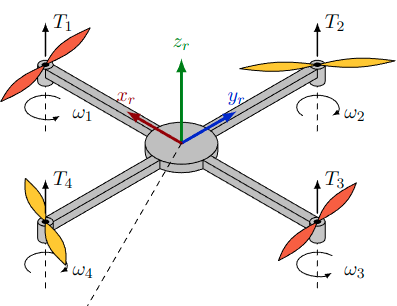
\includegraphics[height=2.5cm, width=3cm]{images/quad_model.png}};
        \node[draw, fill=green!50, text centered, minimum width=3cm, minimum height=1.4cm]
        at ($(drone) + (0.5cm, -3.3cm)$) (pso) {PSO};
        % Arrows
        % Attitude to Drone
        \draw[-stealth] (attitude.east) -- ([yshift=0.25cm] drone.west) 
            node[midway, above] {$\tau_\varphi(\tau_k), \tau_\vartheta(\tau_k), \tau_\psi(\tau_k)$};
        % Position to Attitude
        \draw[-stealth] (position.west) -| (attitude.south) 
            node[near end, left] {$\varphi_d(\tau_k), \vartheta_d(\tau_k), \psi_d(\tau_k)$};
        % Feedback loop from Drone to Attitude
        \draw[-stealth] ([xshift=1cm] drone.east) 
        -- ++(0,1.5cm) % Move up by 1 unit (cm by default in TikZ)
        -- ([yshift=0.5cm] attitude.north) % Move left towards attitude.north with a shift
        -- (attitude.north); % Move down to the exact attitude.north position
        % Incorrect arrow corrected: Drone east side to itself
        \draw (drone.east) -- ++(1cm, 0)
        node[right] {$\mathbf{e}(\tau_k)$};
        % Feedback loop from Drone to Position
        \draw[-stealth] ([xshift=1cm] drone.east) |- ([yshift=0.5cm]position.east);
        % Position to Drone (Thrust, shifted down)
        \draw[-stealth] (position.north) |- ([yshift=-0.25cm] drone.west) 
            node[midway, below right] {$T(\tau_k)$};
        % Position Control Outputs to its East Side
        \draw[-stealth] (pso.west) -- ([yshift=-0.5cm] position.east)
            node[midway, below] {$\mathbf{x}_d(\tau_s), \mathbf{v}_d(\tau_s)$};    
    \end{tikzpicture}}
    \caption{Block diagram of the PID control applied to the PSO algorithm}
    \label{fig:control_PSO}
\end{figure}
COLLEGARE L USCITA DEL MODELLO DEL DRONE CON PSO VOLENDO
Finally, in order to ensure that the drones in the PSO swarm follows
the desired velocity and position commands we integrate the 
PID control described in the previous Section\ref{sec:PID_control} 
with the PSO algorithm described in Section\ref{sec:PSO}.
The block diagram of the complete localization and control 
system is shown in Figure\ref{fig:control_PSO}.
\\

\noindent
\textbf{Important}
\\
Note that the PSO algorithm updates are performed at a sample time 
$\tau_s \neq \tau_k$, where $s \in \mathbb{N}$, which is less 
frequent than the control time step $\tau_k$.
In particular, the PSO algorithm updates once every second, while 
$\tau_k \in \mathbb{R}$.
This implies that at each sample time $\tau_s$ the NSS value is 
evaluated by each $j$-th receiver drone at $\mathbf{p}_{r_j}(\tau_s)$ using 
Eq.\ref{eq:received_signal}.
% SE SI VUOLE DIRE CHE SI USA L EQUAZIONE QUELLA SEMÈLIFICATA BENE SENNO PACE
This value is used to update the personal best position $\mathbf{pbest}_{j}$
of each drone and the group best position $\mathbf{gbest}$ of each group,
which occurs when the current NSS value exceeds previous records. 
Then, the drones update their 2D velocities and positions
as in Eqs.\ref{eq:model_velocity} and \ref{eq:model_position}:
\begin{align}
    \mathbf{v}_{j}(\tau_s+1) &= \omega \mathbf{v}_{j}(\tau_s) 
    + c_1 r_1 \big(\mathbf{pbest}_{j}(\tau_s) - \mathbf{p}_{r_j}(\tau_s)\big) + \notag \\
    &\quad + c_2 r_2 \big(\mathbf{gbest}(\tau_s) - \mathbf{p}_{j}(\tau_s)\big) \label{eq:model_velocity2} \\
    \mathbf{p}_{r_j}(\tau_s + 1) &= \mathbf{p}_{r_j}(\tau_s) + \mathbf{v}_{j}(\tau_s+1) \label{eq:model_position2}
\end{align}
In addition, the velocity clamping in Eq.\ref{eq:velocity_clamping} is performed after
this PSO update.
We also note that the exclusion zone mechanism remains unvaried
and follows the PSO algorithm in the same way.

\noindent
\\
The resulting $\mathbf{v}_{j}(\tau_s+1) = \mathbf{v}_d(\tau_s)$ and $\mathbf{p}_{r_j}(\tau_s + 1) = \mathbf{x}_d(\tau_s)$
are then used as velocity and position desired commands for the PSO, when 
$\tau_s = \tau_k$.
Then, during the next time interval $\Delta \def \tau_{s+1} - \tau_s$ the PID
control algorithm ensures the the the desired position and velocity are reached,
and the drone's movement follows the full dynamics system defined in 
Eq.\ref{eq:final_model_more}:
\begin{equation}
    \dot{\mathbf{\xi}}(\tau_k) = f(\mathbf{\xi}(\tau_k))
\end{equation}
where the drone’s state $\mathbf{\xi}$ is updated at each time step $\tau_k$ in the 
interval $\Delta = \tau_{s+1} - \tau_s$.
Additionally, the control dynamics ensure the 
search space boundary conditions as in
Eq.\ref{eq:boundary_condition}.
This iterative alternation between PSO updates and 
independent drone 
control enables the swarm to balance global 
exploration and local exploitation, 
ensuring efficient source localization and actual 
control inputs.

%\chapter{Experiments}


\backmatter
\cleardoublepage

\newpage
\phantomsection
\addcontentsline{toc}{chapter}{\glossaryname}
\printglossary

\newpage
\phantomsection
\addcontentsline{toc}{chapter}{\bibname}
%\nocite{*} % Uncomment to include uncited references
\printbibliography % Prints the bibliography

\newpage
\phantomsection
\addcontentsline{toc}{section}{Figure}

%\begin{acknowledgments}
\chapter{Ringraziamenti}
SCRIVI QUI I RINGRAZIAMENTI 
%\end{acknowledgments}

\end{document}
